\documentclass[]{elsarticle} %review=doublespace preprint=single 5p=2 column
%%% Begin My package additions %%%%%%%%%%%%%%%%%%%
\usepackage[hyphens]{url}

  \journal{ar\(\chi\)iv} % Sets Journal name


\usepackage{lineno} % add
\providecommand{\tightlist}{%
  \setlength{\itemsep}{0pt}\setlength{\parskip}{0pt}}

\usepackage{graphicx}
\usepackage{booktabs} % book-quality tables
%%%%%%%%%%%%%%%% end my additions to header

\usepackage[T1]{fontenc}
\usepackage{lmodern}
\usepackage{amssymb,amsmath}
\usepackage{ifxetex,ifluatex}
\usepackage{fixltx2e} % provides \textsubscript
% use upquote if available, for straight quotes in verbatim environments
\IfFileExists{upquote.sty}{\usepackage{upquote}}{}
\ifnum 0\ifxetex 1\fi\ifluatex 1\fi=0 % if pdftex
  \usepackage[utf8]{inputenc}
\else % if luatex or xelatex
  \usepackage{fontspec}
  \ifxetex
    \usepackage{xltxtra,xunicode}
  \fi
  \defaultfontfeatures{Mapping=tex-text,Scale=MatchLowercase}
  \newcommand{\euro}{€}
\fi
% use microtype if available
\IfFileExists{microtype.sty}{\usepackage{microtype}}{}
\usepackage[margin=1in]{geometry}
\bibliographystyle{elsarticle-harv}
\ifxetex
  \usepackage[setpagesize=false, % page size defined by xetex
              unicode=false, % unicode breaks when used with xetex
              xetex]{hyperref}
\else
  \usepackage[unicode=true]{hyperref}
\fi
\hypersetup{breaklinks=true,
            bookmarks=true,
            pdfauthor={},
            pdftitle={Gait cycle selection in treadmill running data: Does it matter?},
            colorlinks=false,
            urlcolor=blue,
            linkcolor=magenta,
            pdfborder={0 0 0}}
\urlstyle{same}  % don't use monospace font for urls

\setcounter{secnumdepth}{0}
% Pandoc toggle for numbering sections (defaults to be off)
\setcounter{secnumdepth}{0}


% Pandoc header



\begin{document}
\begin{frontmatter}

  \title{Gait cycle selection in treadmill running data: Does it
matter?}
    \author[Centre for Sport Research]{Aaron S. Fox\corref{1}}
  
    \author[Centre for Sport Research]{Jason Bonacci}
  
    \author[UNSW]{John Warmenhoven}
  
    \author[Centre for Sport Research]{Meghan F. Keast}
  
      \address[Centre for Sport Research]{Centre for Sport Research,
School of Exercise and Nutrition Sciences, Deakin University, Geelong,
Australia}
    \address[UNSW]{School of Engineering and Information Technology,
University of New South Wales, Canberra, Australia}
      \cortext[1]{Corresponding Author}
  
  \begin{abstract}
  Insert abstract\ldots{}
  \end{abstract}
  
 \end{frontmatter}

\hypertarget{introduction}{%
\section{Introduction}\label{introduction}}

\begin{itemize}
\item
  Variety of methods for selecting gait cycles from treadmill-based
  studies of running\ldots{}
\item
  Common process within experimental studies is to collect a certain
  number of gait cycles and use the average of this biomechanical data
  to compute a representative mean for the individual\ldots{}
\item
  There is a need to understand the effect of gait cycle number on
  biomechanical outcome variables from a time cost perspective. We can
  somewhat easily collect a significant number of gait cycles within a
  laboratory environment in a treadmill-based test. Having participants
  settle into a steady state through continuous running over X time
  period is in fact recommended (?). However, there are potential time
  savings to be made within analysis protocols should we need to process
  fewer gait cycles (i.e.~time within IK-like processes, time with data
  cleaning etc.). On the flip side, should only a small number of gait
  cycles result in `unstable' biomechanical variables that aren't
  necessarily representative of an individuals running biomechanics,
  this would suggest a need to collect and process more gait cycles in
  calculating a representative mean for the individual\ldots{}
\end{itemize}

Oliveira and Pirscoveanu({\textbf{???}}) recently examined the typical
number of gait cycles using in running biomechanics studies. On average,
studies used 12 cycles per runner to describe running biomechanics,
while Very few (5 out of 56 studies) used more than 10 cycles
({\textbf{???}}).

Oliveira and Pirscoveanu({\textbf{???}}) subsequently performed a study
investigating the impact of sample size and the number of gait cycles
used on biomechanical outcomes

\textbf{\emph{TODO: outline major findings}}

The findings from their study are, however, specific to overground
running and the specific set of variables analysed (i.e.~foot contact
time, loading rate, peak vertical force, peak braking force, running
speed and foot contact angle). Treadmill-based studies of running are
common across the biomechanical literature \textbf{\emph{ADD REFS}}. It
is plausible that treadmill running may incur a different pattern of
`stability' with respect to the number of gait cycles needed for
analyses, resulting in variable recommendations to those presented by
Oliveira and Pirscoveanu({\textbf{???}}). Further, Oliveira and
Pirscoveanu({\textbf{???}}) did not examine lower limb kinematic
variables commonly used in gait biomechanics studies. These kinematic
variables are presented as both `zero-dimensional' (0D; e.g.~peak
values) and `one-dimensional' (1D; e.g.~time-normalised kinematic
waveform) variables across biomechanical studies \textbf{\emph{ADD
REFS}}. Additional analyses of these common kinematic variables in both
their 0D and 1D forms may, again, yield additional information with
respect to the number of gait cycles required in biomechanical research.

Another limitation to consider is the analysis focused on statistical
significance\ldots not bounds around error measurement?

We sought to understand the impact of the number of gait cycles
selected, along with where these are selected from during a continuous
bout of treadmill running, on biomechanical data and \ldots{} how this
may influence conclusions\ldots{}

First, we used sequential analysis to understand the stability of
biomechanical variables as gait cycle number is increased.

Second, we examined how varying the number of gait cycle samples
impacted the representative mean compared to the entire bout of
continuous treadmill running.

Third, we examined whether sampling gait cycles of varying number from
different sections of an individuals bout of continuous treadmill
running could influence biomechanical outcome variables.

Fourth, we examined whether varying samples of gait cycles could
influence our capacity to detect biomechanical differences between
conditions --- specifically, between running at two different speeds.

\hypertarget{dataset}{%
\section{Dataset}\label{dataset}}

We used the public dataset of treadmill running biomechanics from
Fukuchi et al.({\textbf{???}}). The specifics of this dataset can be
found in the associated paper ({\textbf{???}}). Briefly, this dataset
contains lower-extremity kinematics and kinetics of 28 regular runners
(27 male, 1 female; age = 34.8 ± 6.7 years; height = 176.0 ± 6.8 cm;
mass = 69.6 ± 7.7 kg; running experience = 8.5 ± 7.0 years; running pace
= 4.1 ± 0.4 min/km) ({\textbf{???}}). Running kinematics were collected
using a 12-camera 3D motion capture system (Raptor-4, Motion Analysis,
Santa Rosa, CA, United States) and ground reaction force (GRF) data via
an instrumented dual-belt treadmill (FIT, Bertec, Columbus, OH, United
States) ({\textbf{???}}). Participants ran on the treadmill at three
designated speeds (2.5m·s\textsuperscript{-1},
3.5m·s\textsuperscript{-1} and 4.5m·s\textsuperscript{-1}), during which
a three-minute accommodation period was provided followed by a 30-second
data collection period ({\textbf{???}}).

We processed the experimental data from Fukuchi et al.({\textbf{???}})
using OpenSim 4.0 ({\textbf{???}}). Segment geometry of the generic
musculoskeletal model of the pelvis and lower limb provided by Lai et
al.({\textbf{???}}) were scaled for each participant using their static
calibration trial, which was also used as a reference for adjusting
marker positions on the model. Lower limb joint angles were calculated
using filtered (10Hz low-pass 4\textsuperscript{th} order Butterworth)
marker trajectory data within inverse kinematics analysis. GRF data were
also filtered using the same cut-off frequency and filter. The filtering
procedures reflected those originally performed by Fukuchi et
al.({\textbf{???}}). Foot strike and toe-off events were determined when
the vertical GRF crossed a 20N threshold, also in line with the original
work on this dataset ({\textbf{???}}).

Kinematic variables common to gait biomechanics studies (i.e.~hip
flexion/extension, hip adduction/abduction, hip internal/external
rotation, knee flexion and ankle plantarflexion/dorsiflexion) were
extracted from the right limb for all participants. Data between
consecutive foot strikes were extracted and time-normalised to 0-100\%
of the gait cycle. The time-normalised one-dimensional (1D) curves were
used in subsequent 1D analyses, while a set of peak variables (hip
flexion, hip adduction, hip internal rotation, knee flexion, ankle
dorsiflexion) were calculated and extracted for the zero-dimensional
(0D) analyses.

\hypertarget{how-many-gait-cycles-are-required-to-generate-stable-kinematic-data}{%
\section{How many gait cycles are required to generate `stable'
kinematic
data?}\label{how-many-gait-cycles-are-required-to-generate-stable-kinematic-data}}

We used sequential analysis to examine the threshold for the number of
gait cycles required to reach a `stable' representative mean from the
30-second bout of treadmill running. Sequential analysis was
individually applied across the different running speeds and kinematic
variables (both 0D and 1D variants). We used multiple bandwidths to
examine varying thresholds of `stability.' This included the typical ±
25\% of one standard deviation from the target mean, in line with
existing studies applying sequential analysis to biomechanical data
\textbf{\emph{{[}\ldots ADD REFS\ldots{]}}}; but also expanded this to ±
50\%, 75\% and 100\% of one standard deviation from the target mean.
These additional analyses were undertaken to provide various thresholds
for which researchers can apply to their own studies. For 0D variables,
the sequential discrete data points across all gait cycles from each
participant were averaged to create the target stability value, from
which the various standard deviation bandwidths were applied. To be
considered `stable,' a 0D variable had to fall and remain within the
bandwidth for the remaining gait cycles within the treadmill bout. For
1D variables, the same technique was applied to each time-normalised
point along the continuous kinematic waveform. To be considered
`stable,' all points along the 1D kinematic waveform had to fall and
remain within the bandwidth for the remaining gait cycles within the
treadmill bout. The number of gait cycles where stability was reached
across the various running speeds, kinematic variables and stability
thresholds were extracted and descriptive statistics (i.e.~mean, median,
inter-quartile ranges, total range) were calculated. The proportion of
participants reaching stability at each gait cycle number was also
calculated.

\emph{TODO: add results for this section here\ldots{}}

\begin{itemize}
\tightlist
\item
  Sequential analysis revealed\ldots{}
\item
  Stability reached earlier with 0D vs.~1D variables (see boxplot) --
  Also more steadier build up of participants who reached stability from
  0D to 1D (i.e.~the lower bound for the number of cycles required for
  1D variables was higher -- see line plot)
\item
  Stability reached with fewer gait cycles with an altered stability
  boundary (i.e.~0.25 SD to 1SD)
\item
  No.~of gait cycles to reach stability seemed relatively independent of
  variable type (consistent number of gait cycles required) irrespective
  of the lower limb variable considered
\item
  Wide ranges for reaching stability across individuals (e.g.~some
  required very few, \textless{} 10; others required a large number of
  gait cycles \textgreater{} 30) -- this was dependent on the threshold
  though
\item
  Seemed to be a slight shift for the proportion of participants
  reaching stability as speed increased (see line plots) -- slight shift
  to the right of the curves for the number of participants reaching
  stability as speed increased
\item
  Very few participants reached stability with \textless{} 20 gait
  cycles for 1D variables at 0.25\% SD, pretty strict criteria for this
  given whole gait cycle was used though
\end{itemize}

Zero-dimensional kinematic variables reached `stable' values with fewer
gait cycles compared to 1D variables irrespective of the running speed
or stability threshold used (see Figure \ref{fig:boxplotStability})

\begin{figure}

{\centering 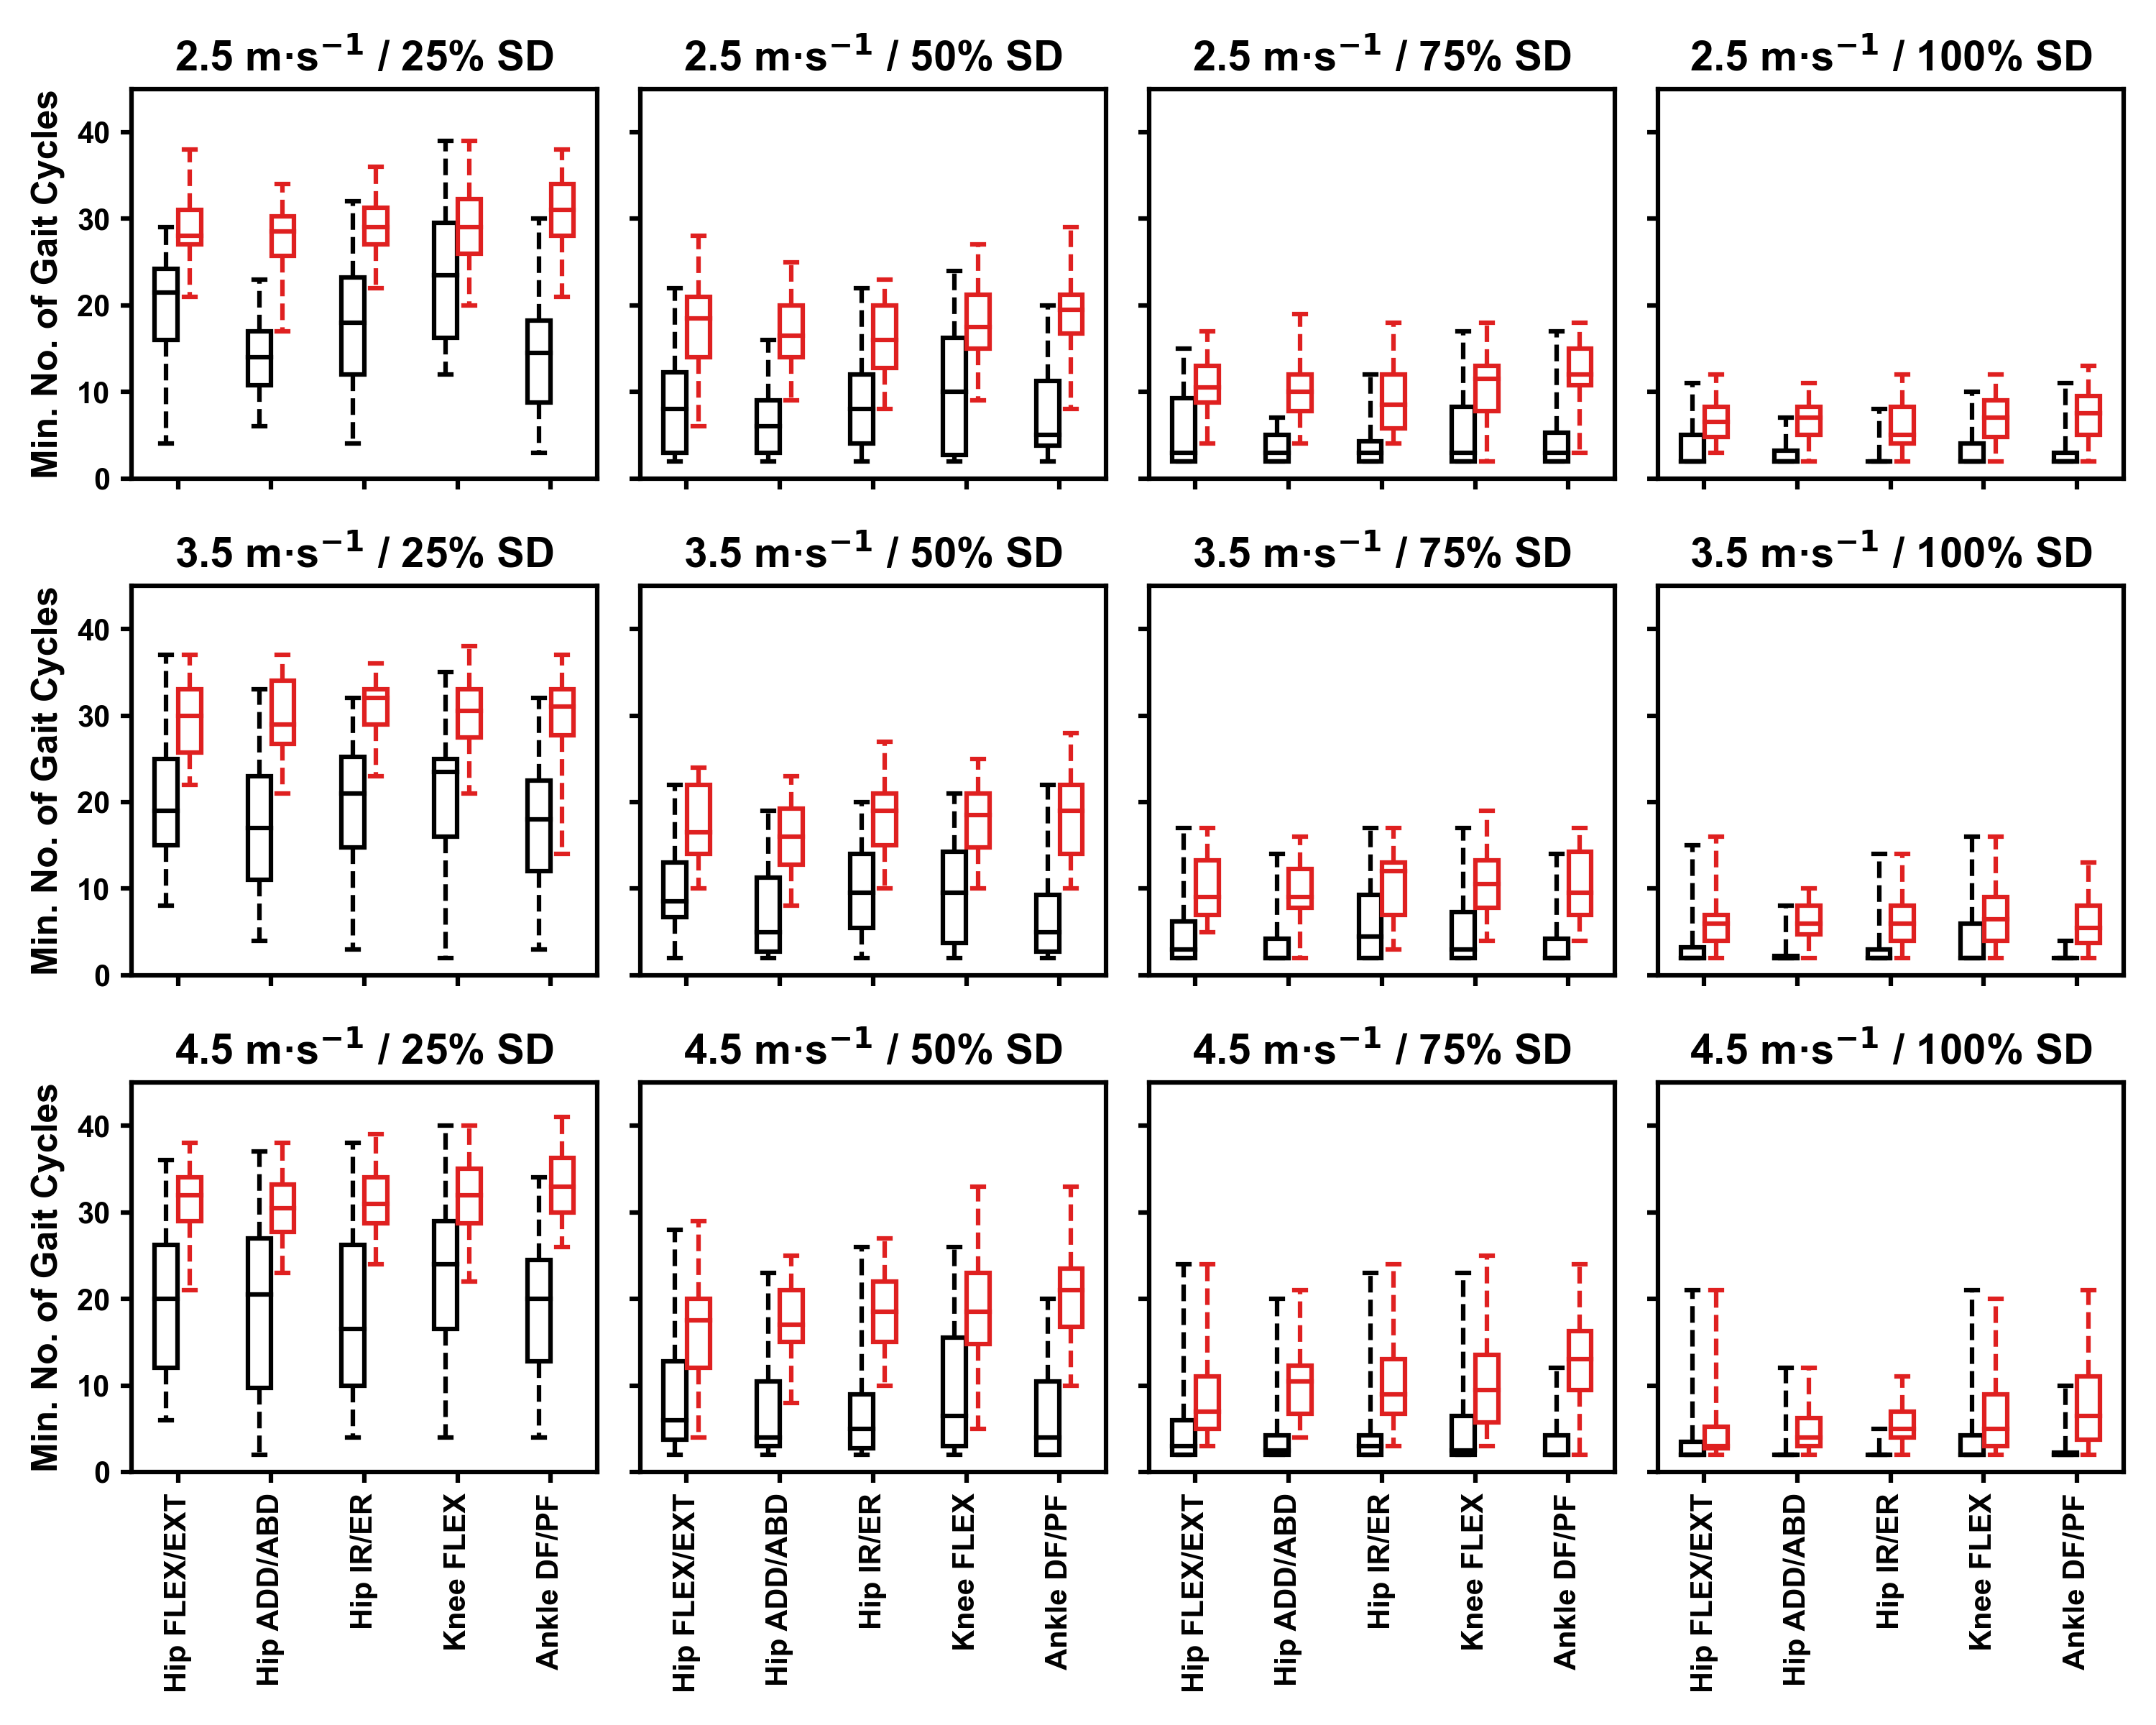
\includegraphics[width=1\linewidth]{D:/+GitRepos+/biomech-trial-selection/Analysis/SequentialAnalysis/Figures/Boxplot_NoGaitCycles_Stability} 

}

\caption{Number of gait cycles required to produce a 'stable' value at various speeds (i.e. rows; 2.5m·s$^{-1}$, 3.5m·s$^{-1}$ and 4.5m·s$^{-1}$) and stability thresholds (i.e. columns; 25$\%$, 50$\%$, 75$\%$ and 100$\%$ of one standard deviation [SD] from the stable mean) for zero-dimensional (0D; black) and one-dimensional (1D; red) kinematic variables. Horizontal lines within boxes equate to the median value, boxes indicate the 25$^{th}$ to 75$^{th}$ percentile, and whiskers indicate the range. Shaded violins are included to illustrate the distribution of values.}\label{fig:boxplotStability}
\end{figure}

\begin{figure}

{\centering 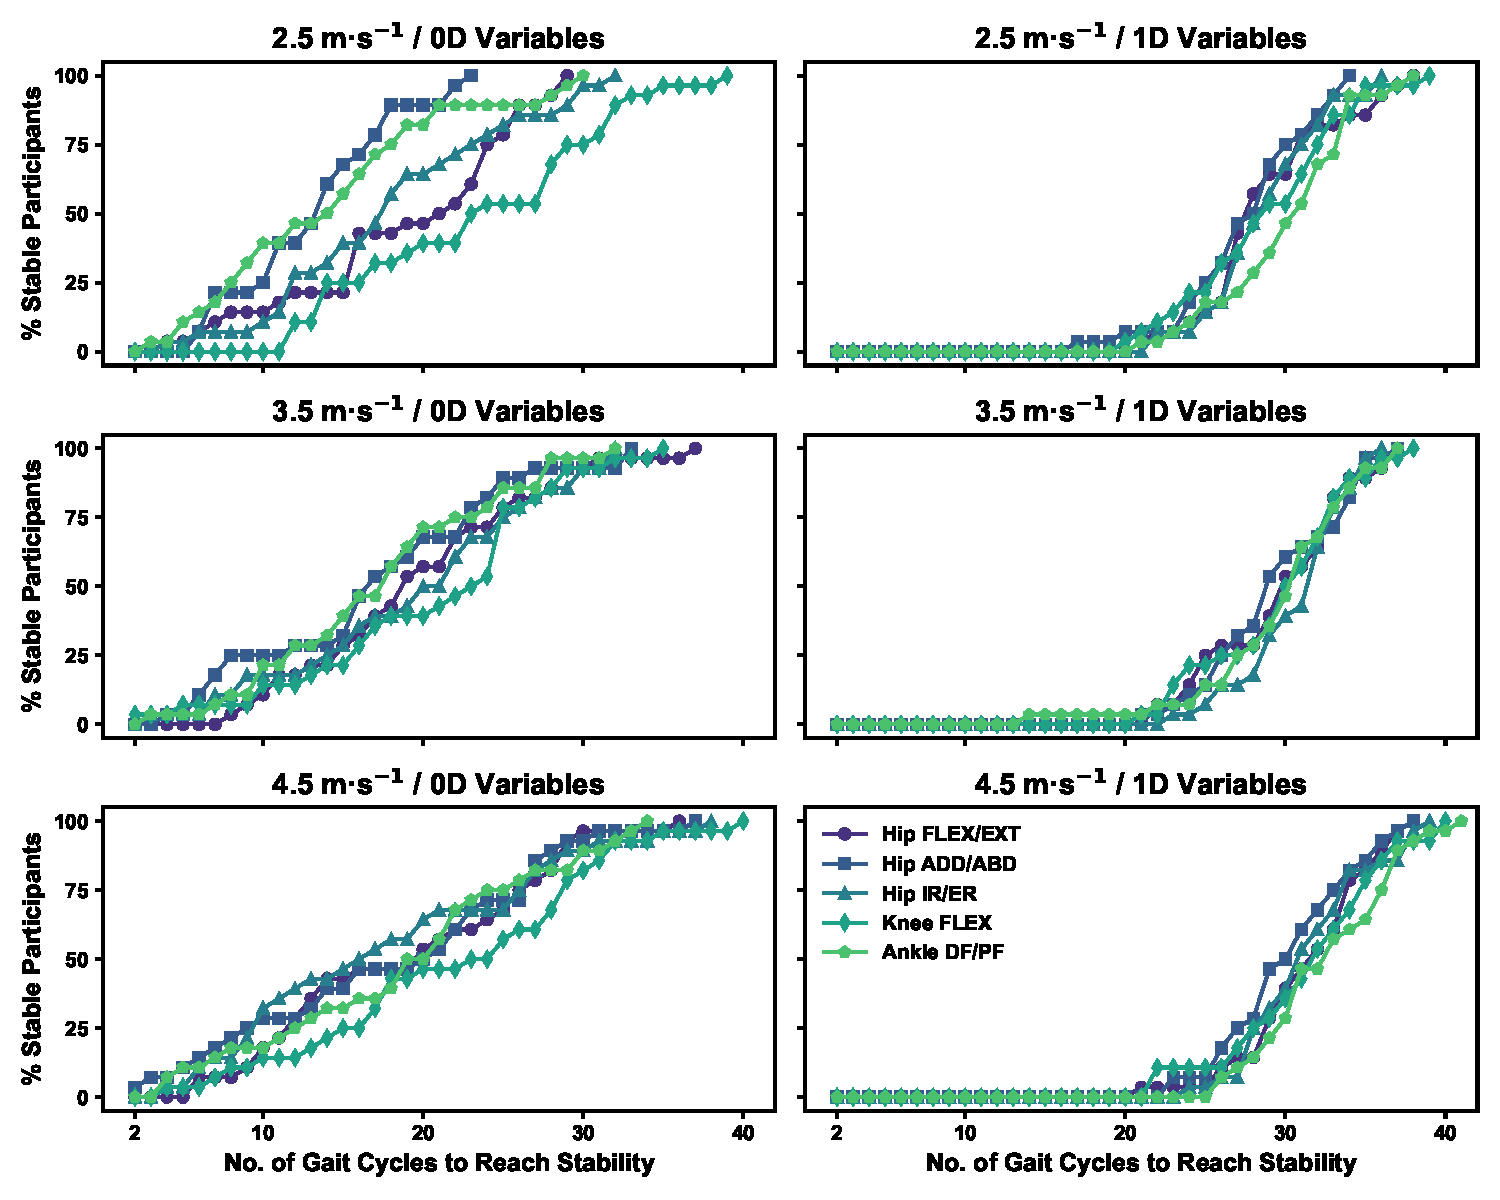
\includegraphics[width=1\linewidth]{D:/+GitRepos+/biomech-trial-selection/Analysis/SequentialAnalysis/Figures/LinePlot_StableProportion_25perSD} 

}

\caption{Proportion of participants displaying 'stable' values for zero-dimensional (0D; left column) and one-dimensional (1D; right column) kinematic variables at various speeds (i.e. rows; 2.5m·s$^{-1}$, 3.5m·s$^{-1}$ and 4.5m·s$^{-1}$) using a stability threshold of 25$\%$ of one standard deviation from the stable mean.}\label{fig:stableParticipants25}
\end{figure}

\begin{figure}

{\centering 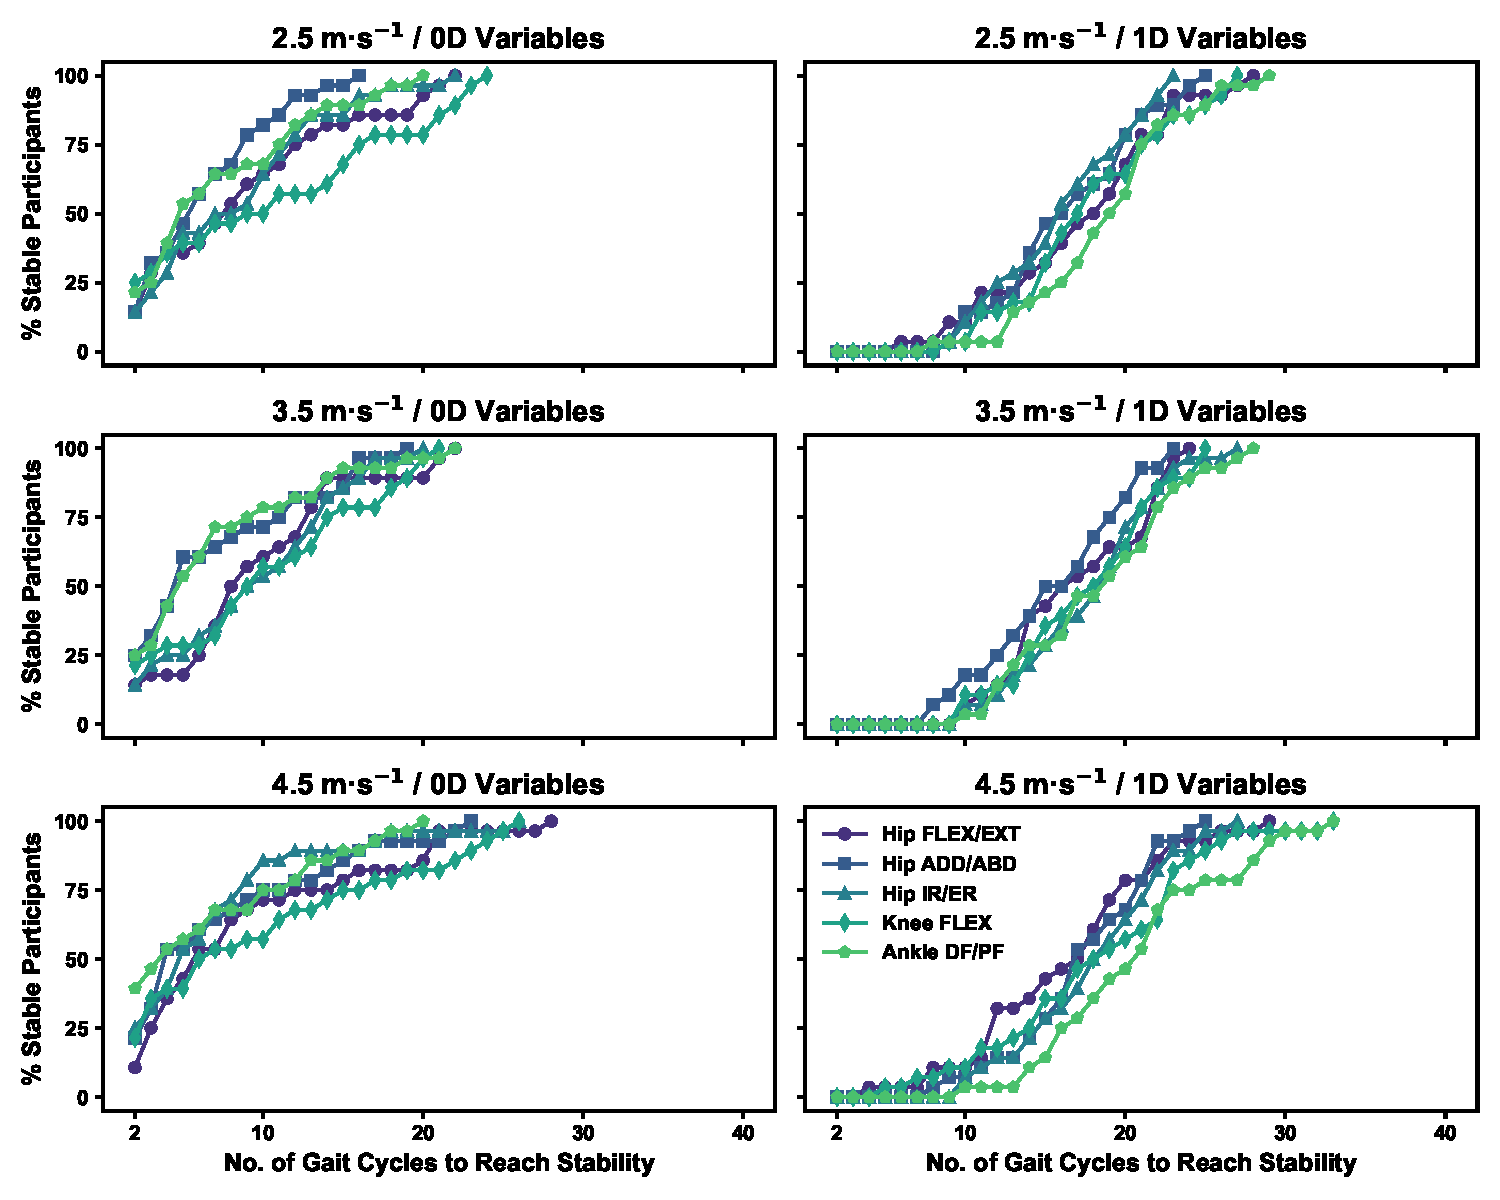
\includegraphics[width=1\linewidth]{D:/+GitRepos+/biomech-trial-selection/Analysis/SequentialAnalysis/Figures/LinePlot_StableProportion_50perSD} 

}

\caption{Proportion of participants displaying 'stable' values for zero-dimensional (0D; left column) and one-dimensional (1D; right column) kinematic variables at various speeds (i.e. rows; 2.5m·s$^{-1}$, 3.5m·s$^{-1}$ and 4.5m·s$^{-1}$) using a stability threshold of 50$\%$ of one standard deviation from the stable mean.}\label{fig:stableParticipants50}
\end{figure}

\begin{figure}

{\centering 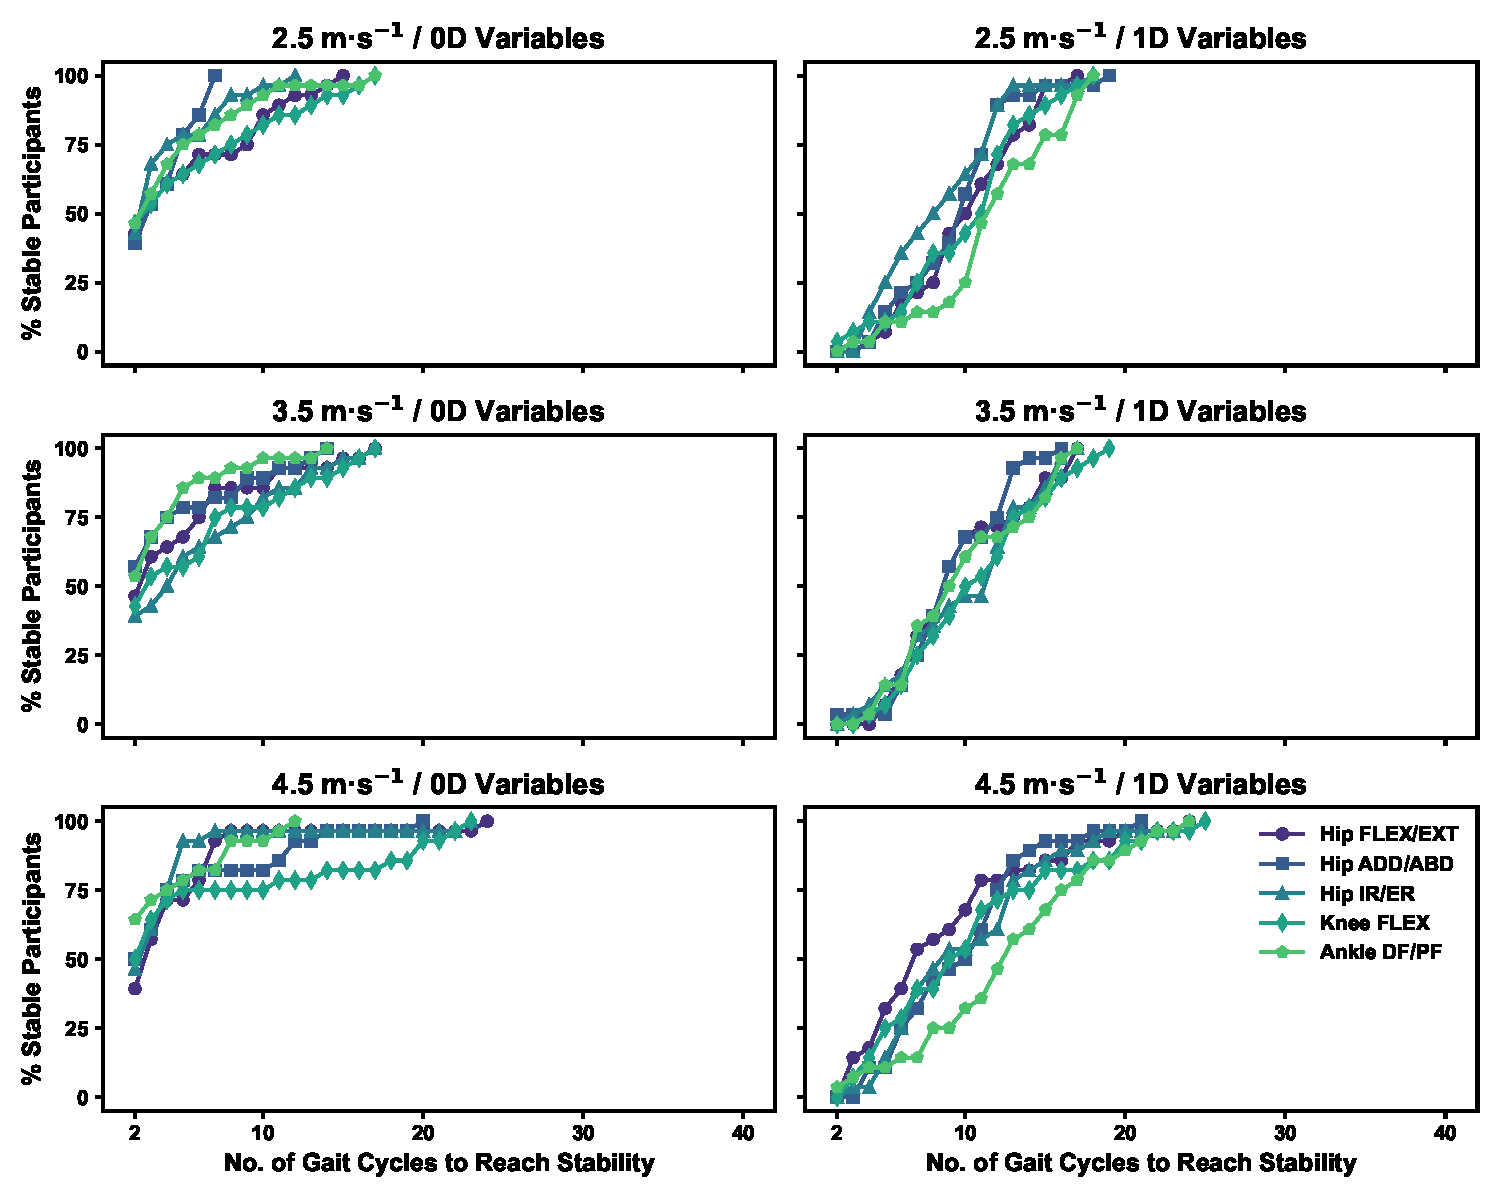
\includegraphics[width=1\linewidth]{D:/+GitRepos+/biomech-trial-selection/Analysis/SequentialAnalysis/Figures/LinePlot_StableProportion_75perSD} 

}

\caption{Proportion of participants displaying 'stable' values for zero-dimensional (0D; left column) and one-dimensional (1D; right column) kinematic variables at various speeds (i.e. rows; 2.5m·s$^{-1}$, 3.5m·s$^{-1}$ and 4.5m·s$^{-1}$) using a stability threshold of 75$\%$ of one standard deviation from the stable mean.}\label{fig:stableParticipants75}
\end{figure}

\begin{figure}

{\centering 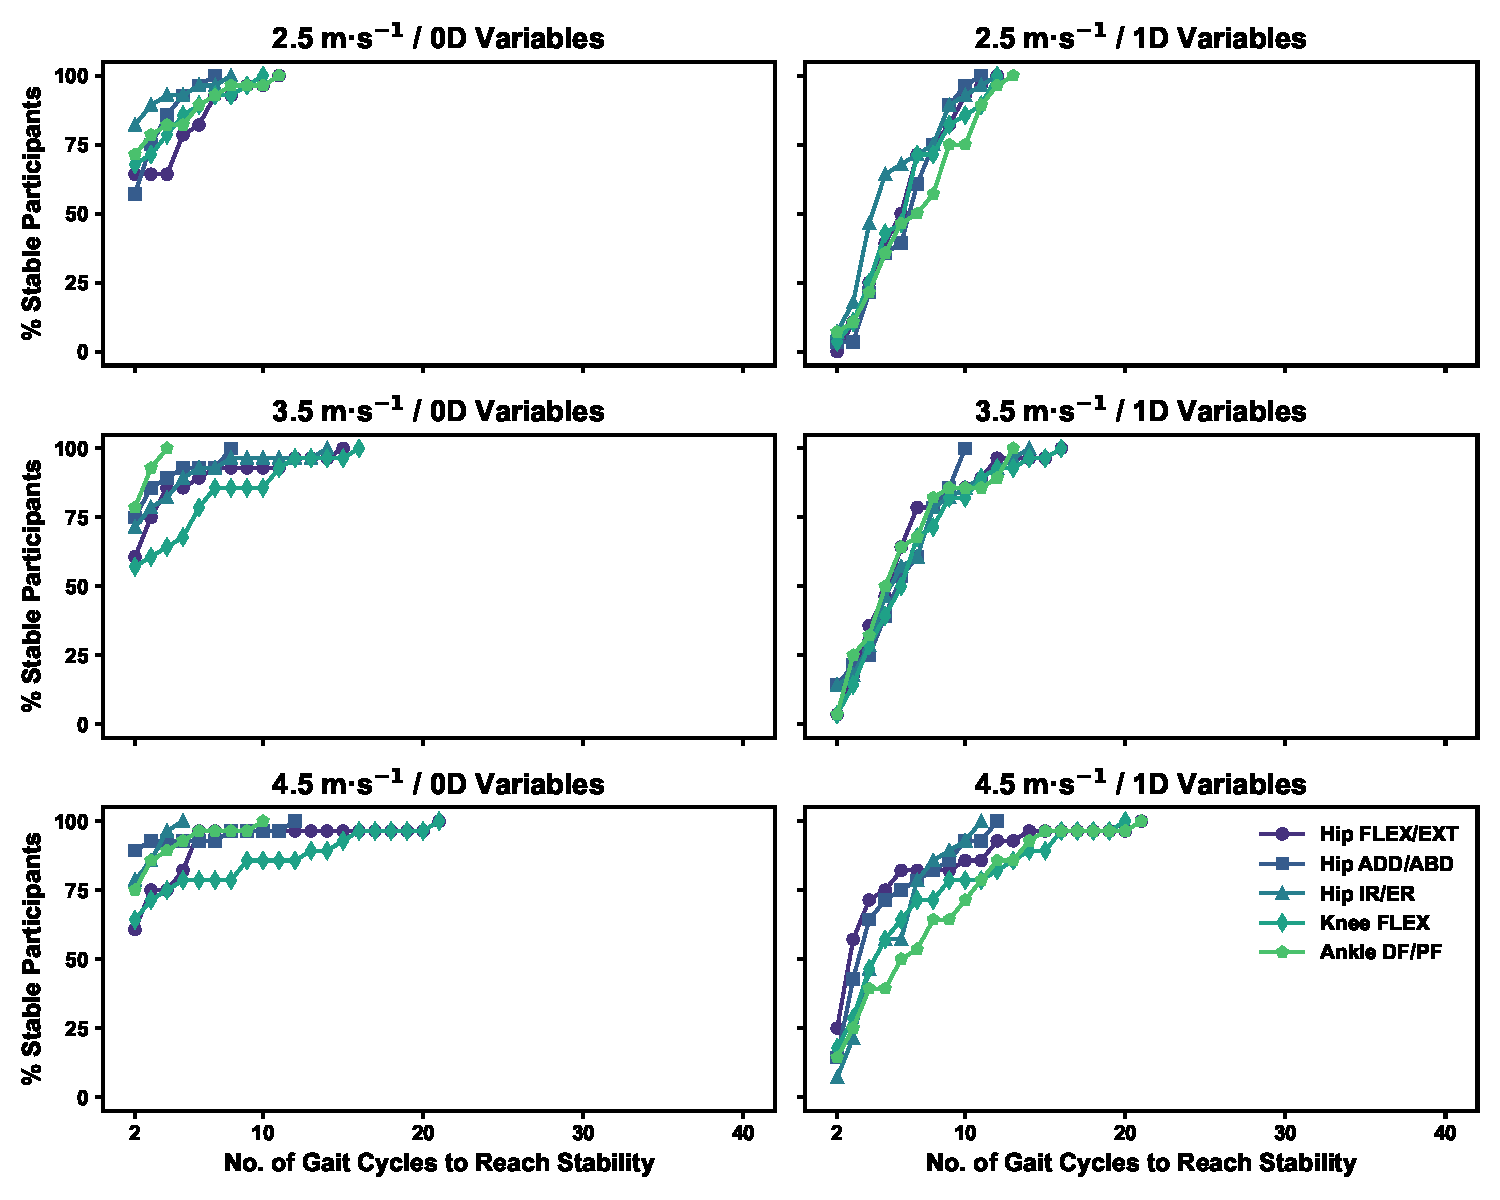
\includegraphics[width=1\linewidth]{D:/+GitRepos+/biomech-trial-selection/Analysis/SequentialAnalysis/Figures/LinePlot_StableProportion_100perSD} 

}

\caption{Proportion of participants displaying 'stable' values for zero-dimensional (0D; left column) and one-dimensional (1D; right column) kinematic variables at various speeds (i.e. rows; 2.5m·s$^{-1}$, 3.5m·s$^{-1}$ and 4.5m·s$^{-1}$) using a stability threshold of 100$\%$ of one standard deviation from the stable mean.}\label{fig:stableParticipants100}
\end{figure}

\hypertarget{how-does-the-number-of-gait-cycles-used-impact-the-representative-kinematic-mean}{%
\section{How does the number of gait cycles used impact the
representative kinematic
mean?}\label{how-does-the-number-of-gait-cycles-used-impact-the-representative-kinematic-mean}}

\emph{TODO: add methods\ldots{}}

\begin{figure}

{\centering 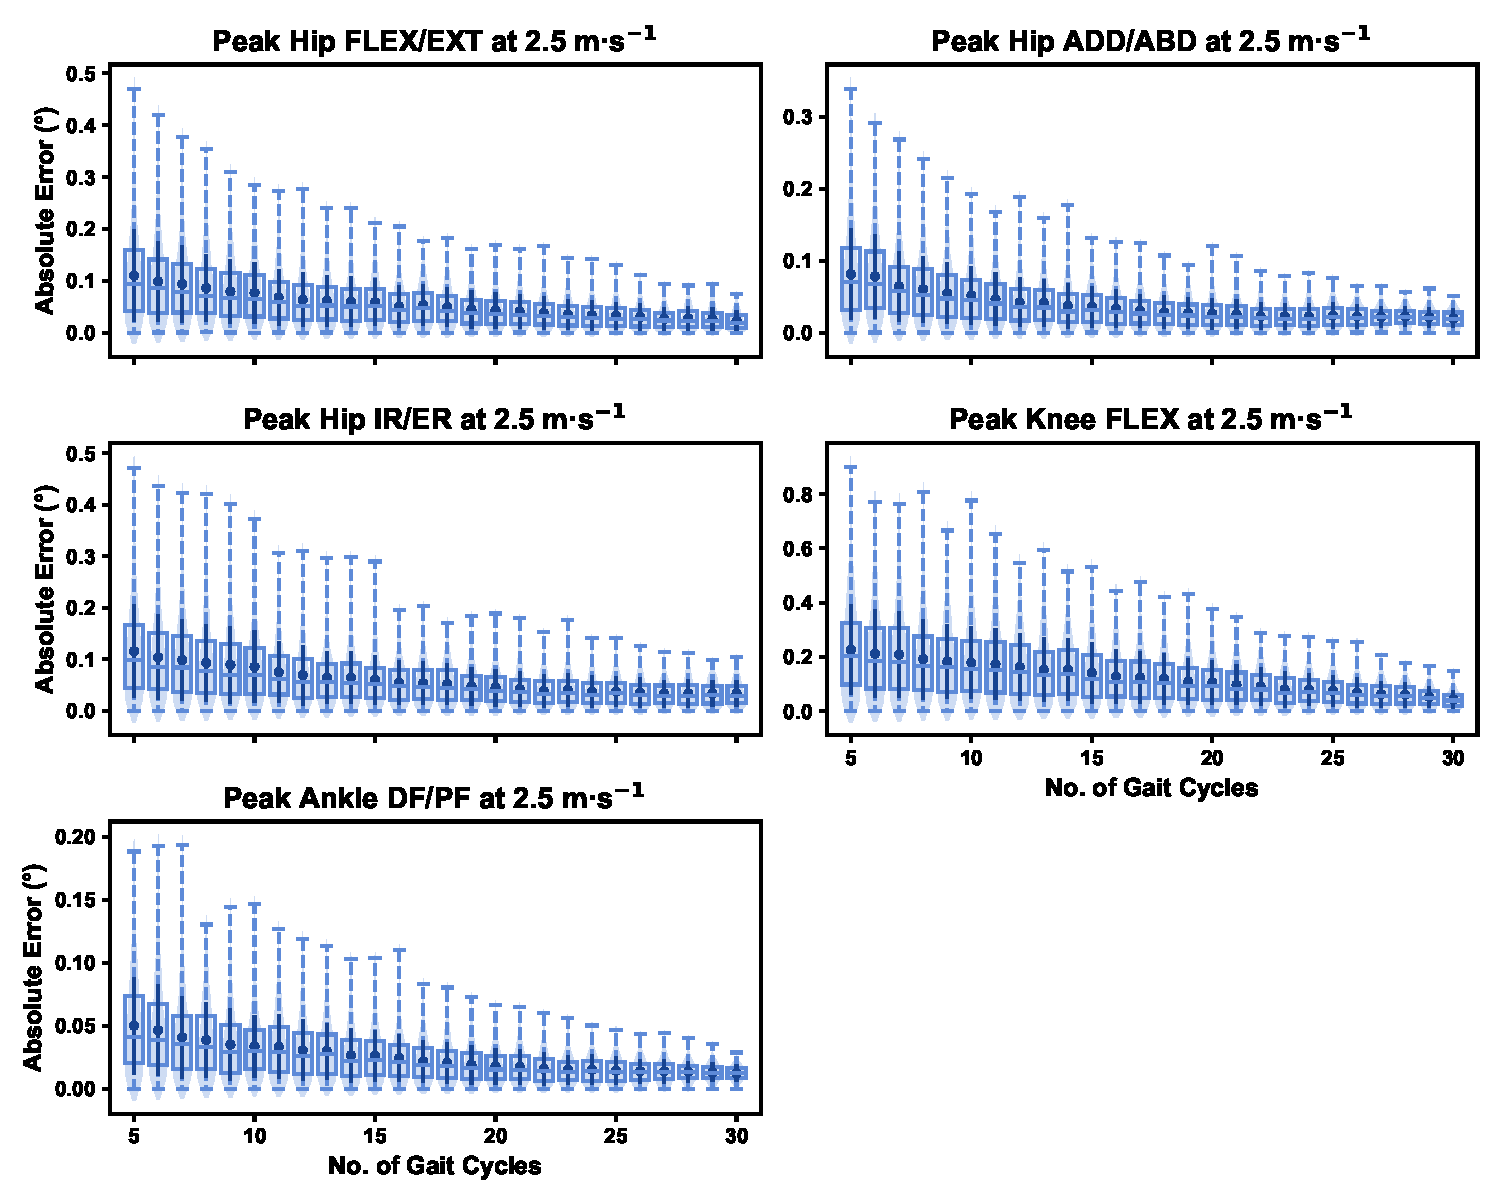
\includegraphics[width=1\linewidth]{D:/+GitRepos+/biomech-trial-selection/Analysis/GroundTruthComp/Figures/AbsoluteError_NoGaitCycle_runT25_0D} 

}

\caption{Absolute error in peak kinematic variables (i.e. zero-dimensional [0D]) when running at 2.5m·s$^{-1}$ using a subset of gait cycles versus all gait cycles from the 30 second treadmill bout. Horizontal lines within boxes equate to the median value, boxes indicate the 25$^{th}$ to 75$^{th}$ percentile, and whiskers indicate the range. Shaded violins are included to illustrate the distribution of values. FLEX — flexion; EXT — extension; ADD — adduction; ABD — abduction; IR — internal rotation; ER — external rotation; DF — dorsiflexion; PF — plantarflexion.}\label{fig:groundTruthError_runT25_0D}
\end{figure}

\begin{figure}

{\centering 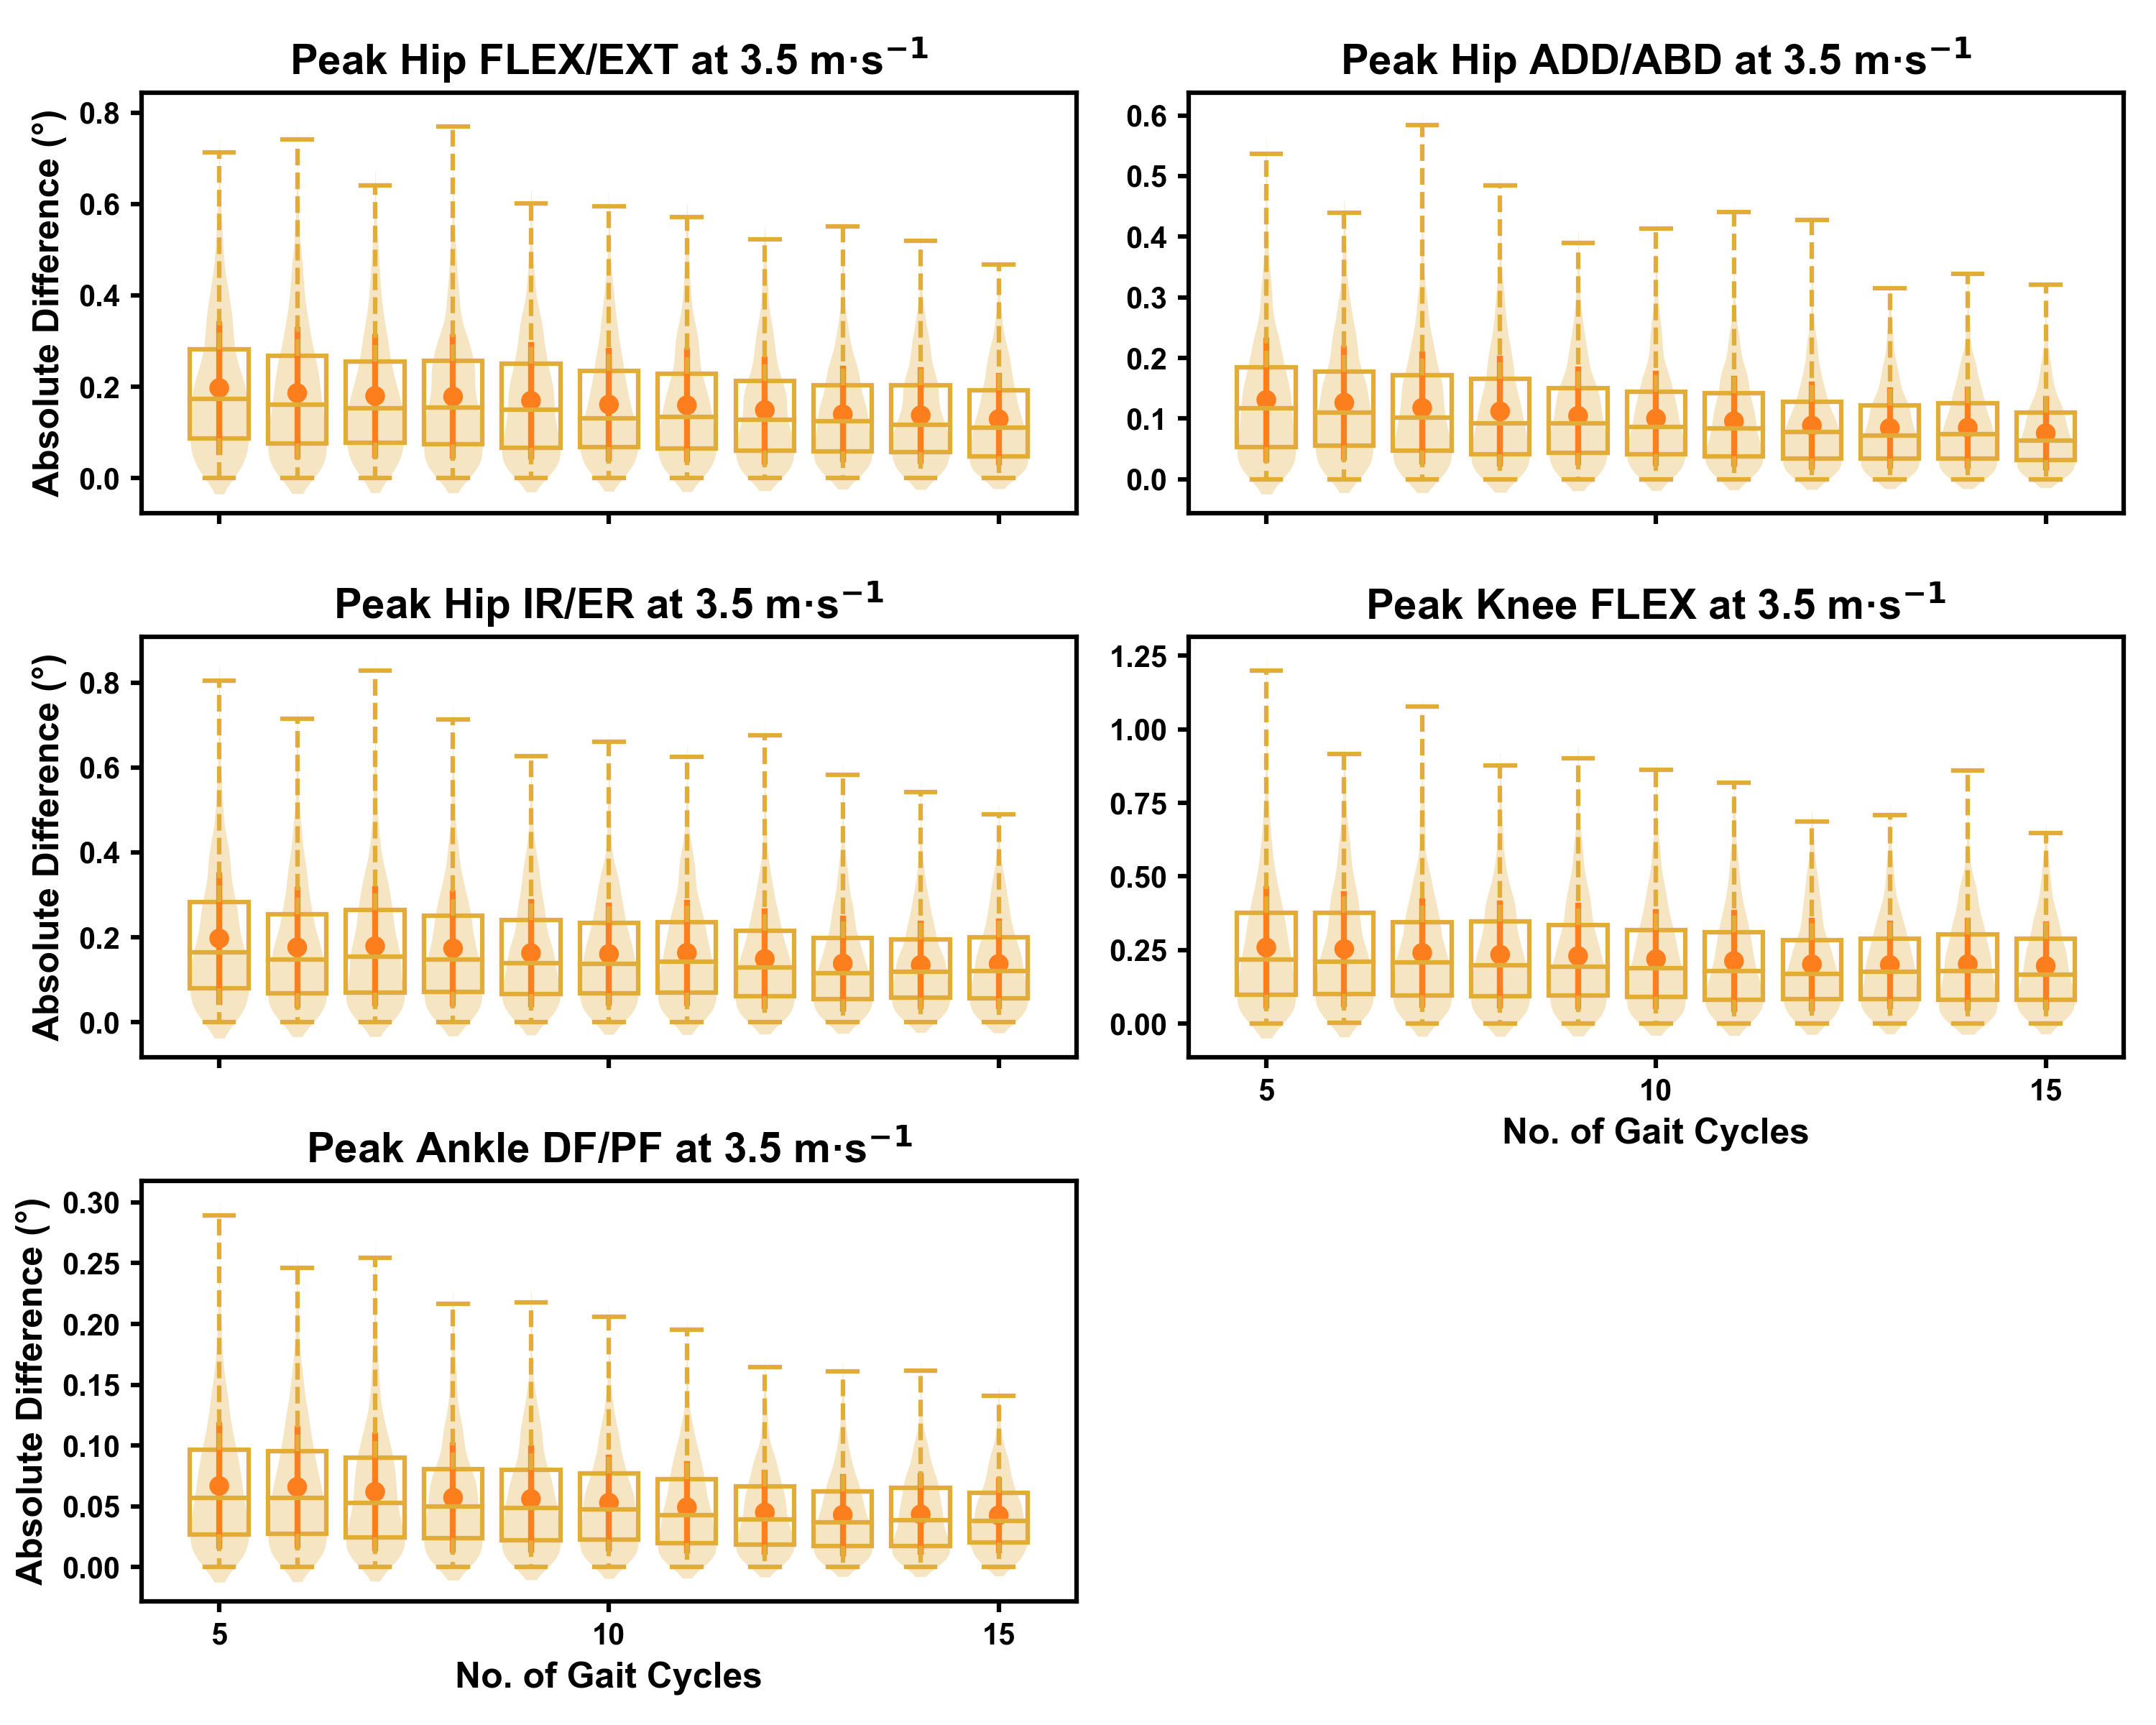
\includegraphics[width=1\linewidth]{D:/+GitRepos+/biomech-trial-selection/Analysis/GroundTruthComp/Figures/AbsoluteError_NoGaitCycle_runT35_0D} 

}

\caption{Absolute error in peak kinematic variables (i.e. zero-dimensional [0D]) when running at 3.5m·s$^{-1}$ using a subset of gait cycles versus all gait cycles from the 30 second treadmill bout. Horizontal lines within boxes equate to the median value, boxes indicate the 25$^{th}$ to 75$^{th}$ percentile, and whiskers indicate the range. Shaded violins are included to illustrate the distribution of values. FLEX — flexion; EXT — extension; ADD — adduction; ABD — abduction; IR — internal rotation; ER — external rotation; DF — dorsiflexion; PF — plantarflexion.}\label{fig:groundTruthError_runT35_0D}
\end{figure}

\begin{figure}

{\centering 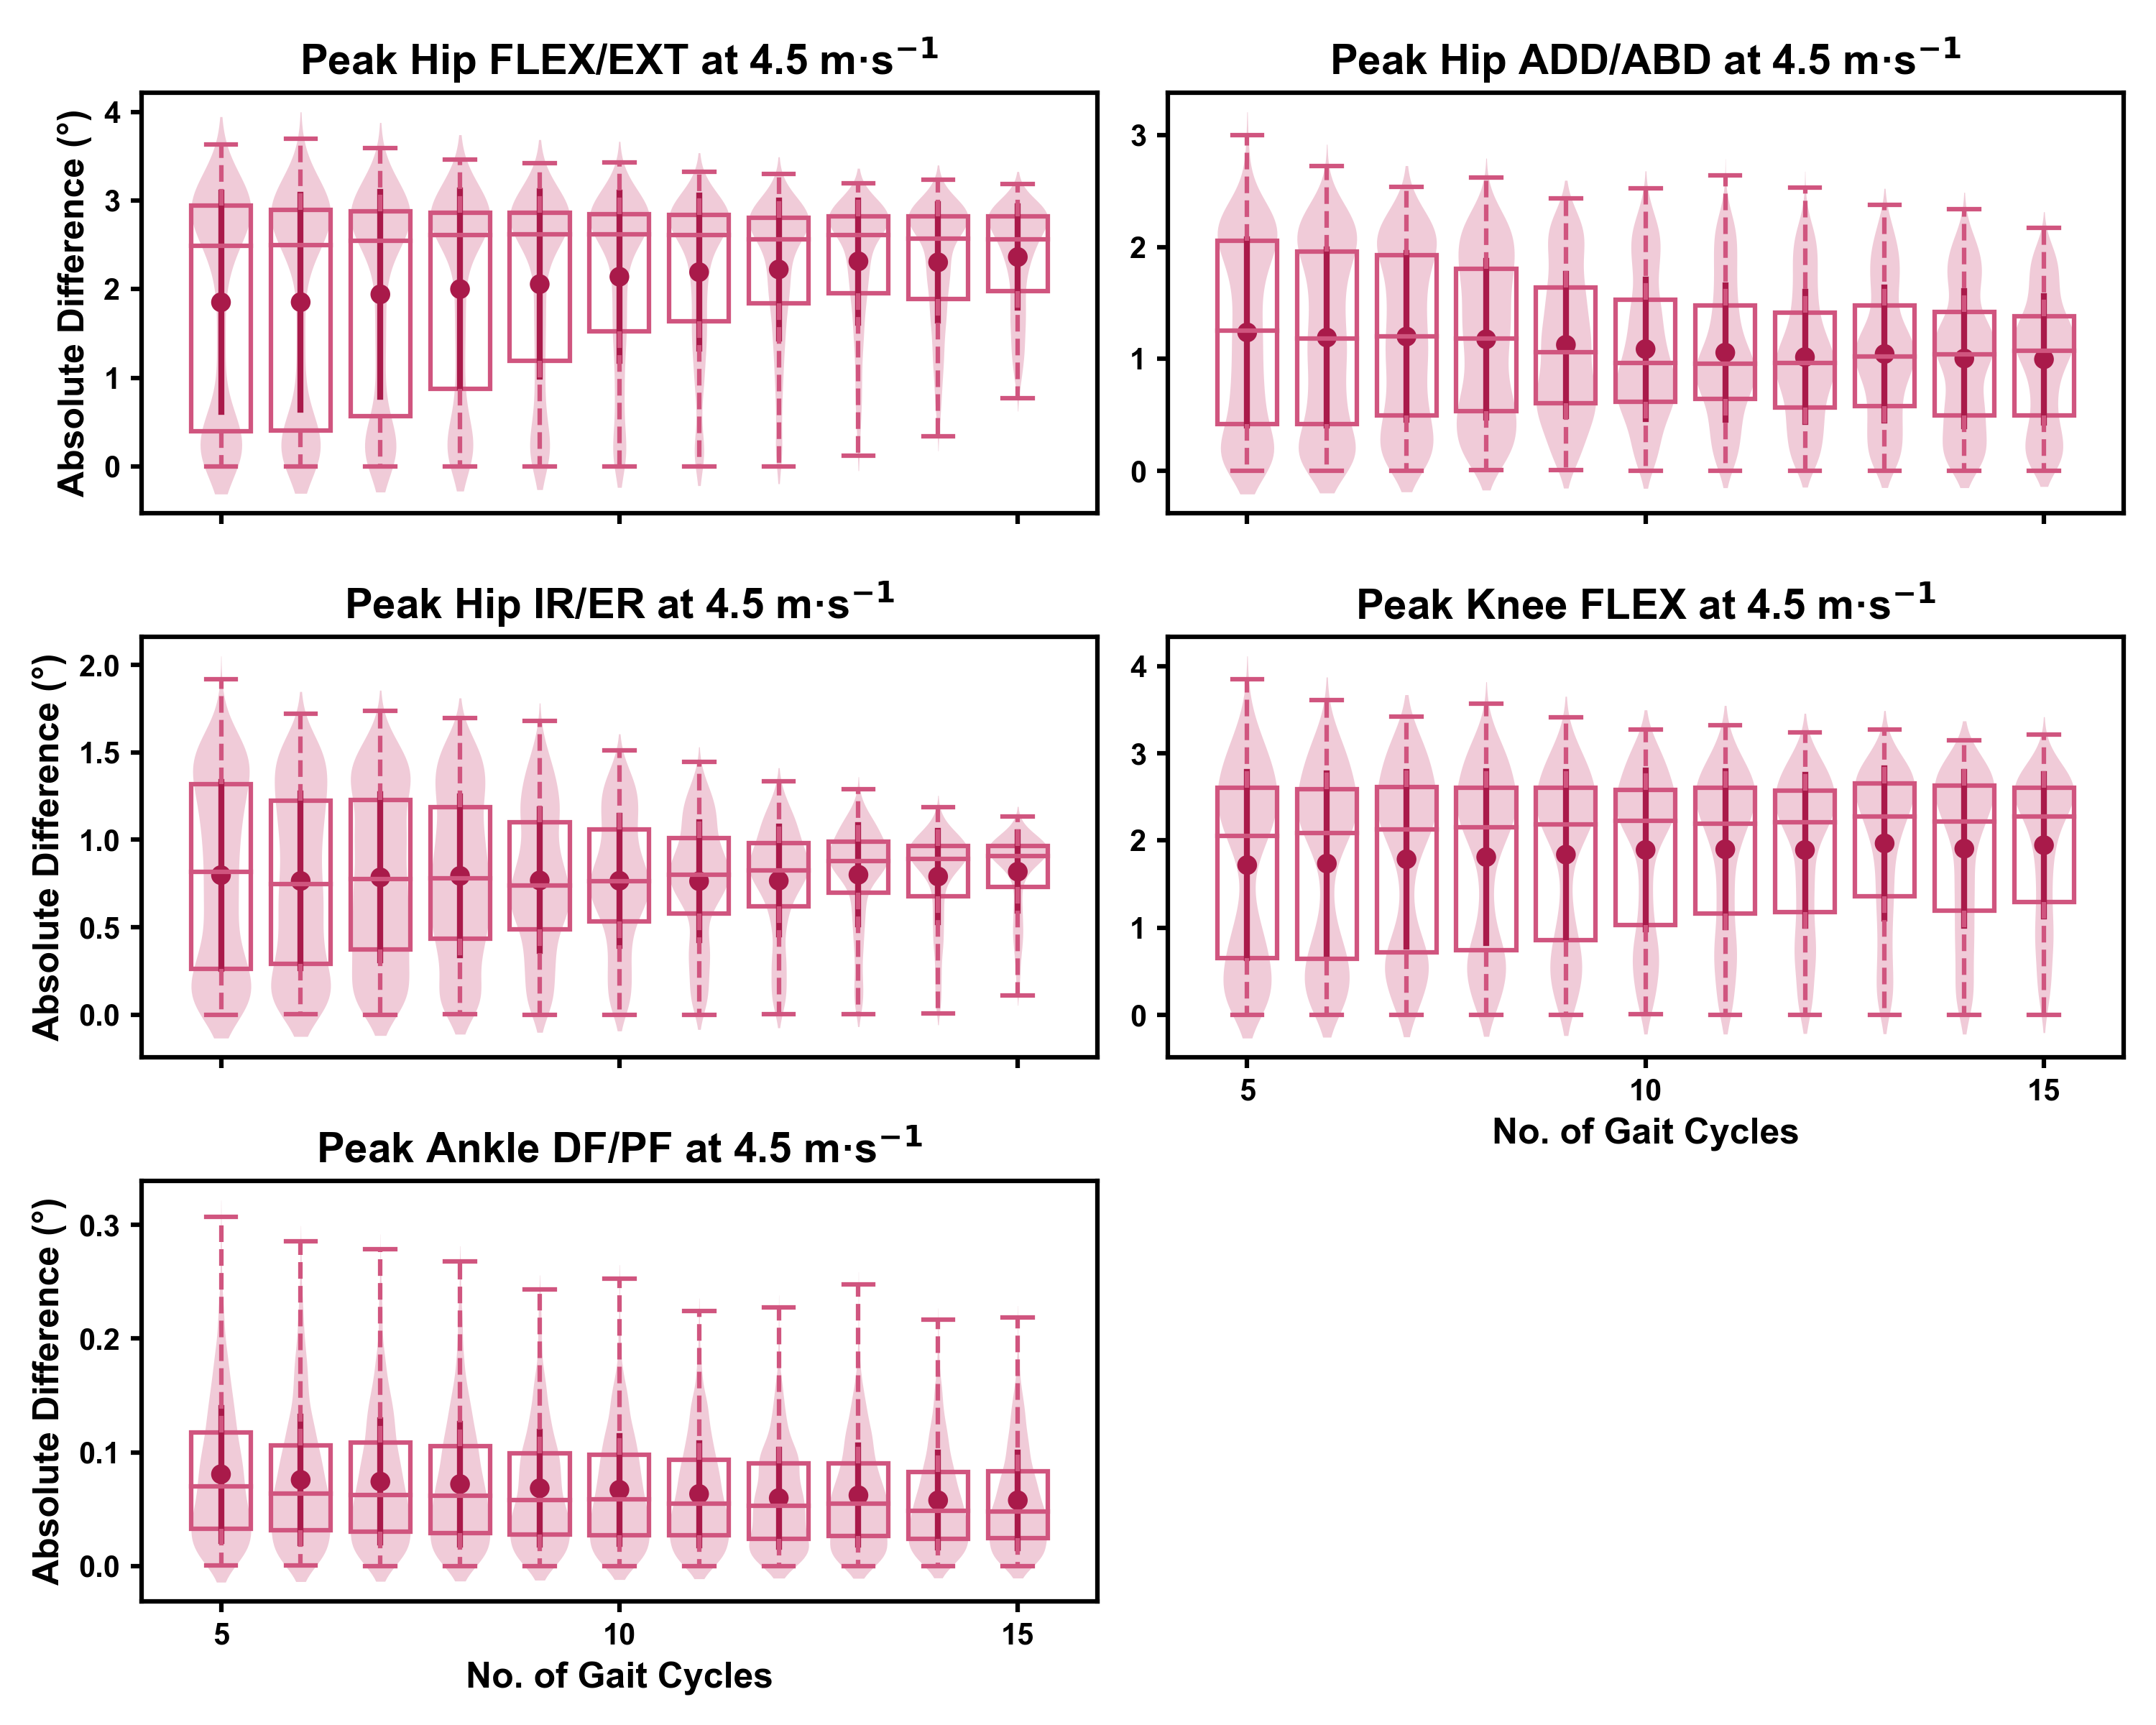
\includegraphics[width=1\linewidth]{D:/+GitRepos+/biomech-trial-selection/Analysis/GroundTruthComp/Figures/AbsoluteError_NoGaitCycle_runT45_0D} 

}

\caption{Absolute error in peak kinematic variables (i.e. zero-dimensional [0D]) when running at 4.5m·s$^{-1}$ using a subset of gait cycles versus all gait cycles from the 30 second treadmill bout. Horizontal lines within boxes equate to the median value, boxes indicate the 25$^{th}$ to 75$^{th}$ percentile, and whiskers indicate the range. Shaded violins are included to illustrate the distribution of values. FLEX — flexion; EXT — extension; ADD — adduction; ABD — abduction; IR — internal rotation; ER — external rotation; DF — dorsiflexion; PF — plantarflexion.}\label{fig:groundTruthError_runT45_0D}
\end{figure}

\begin{figure}

{\centering 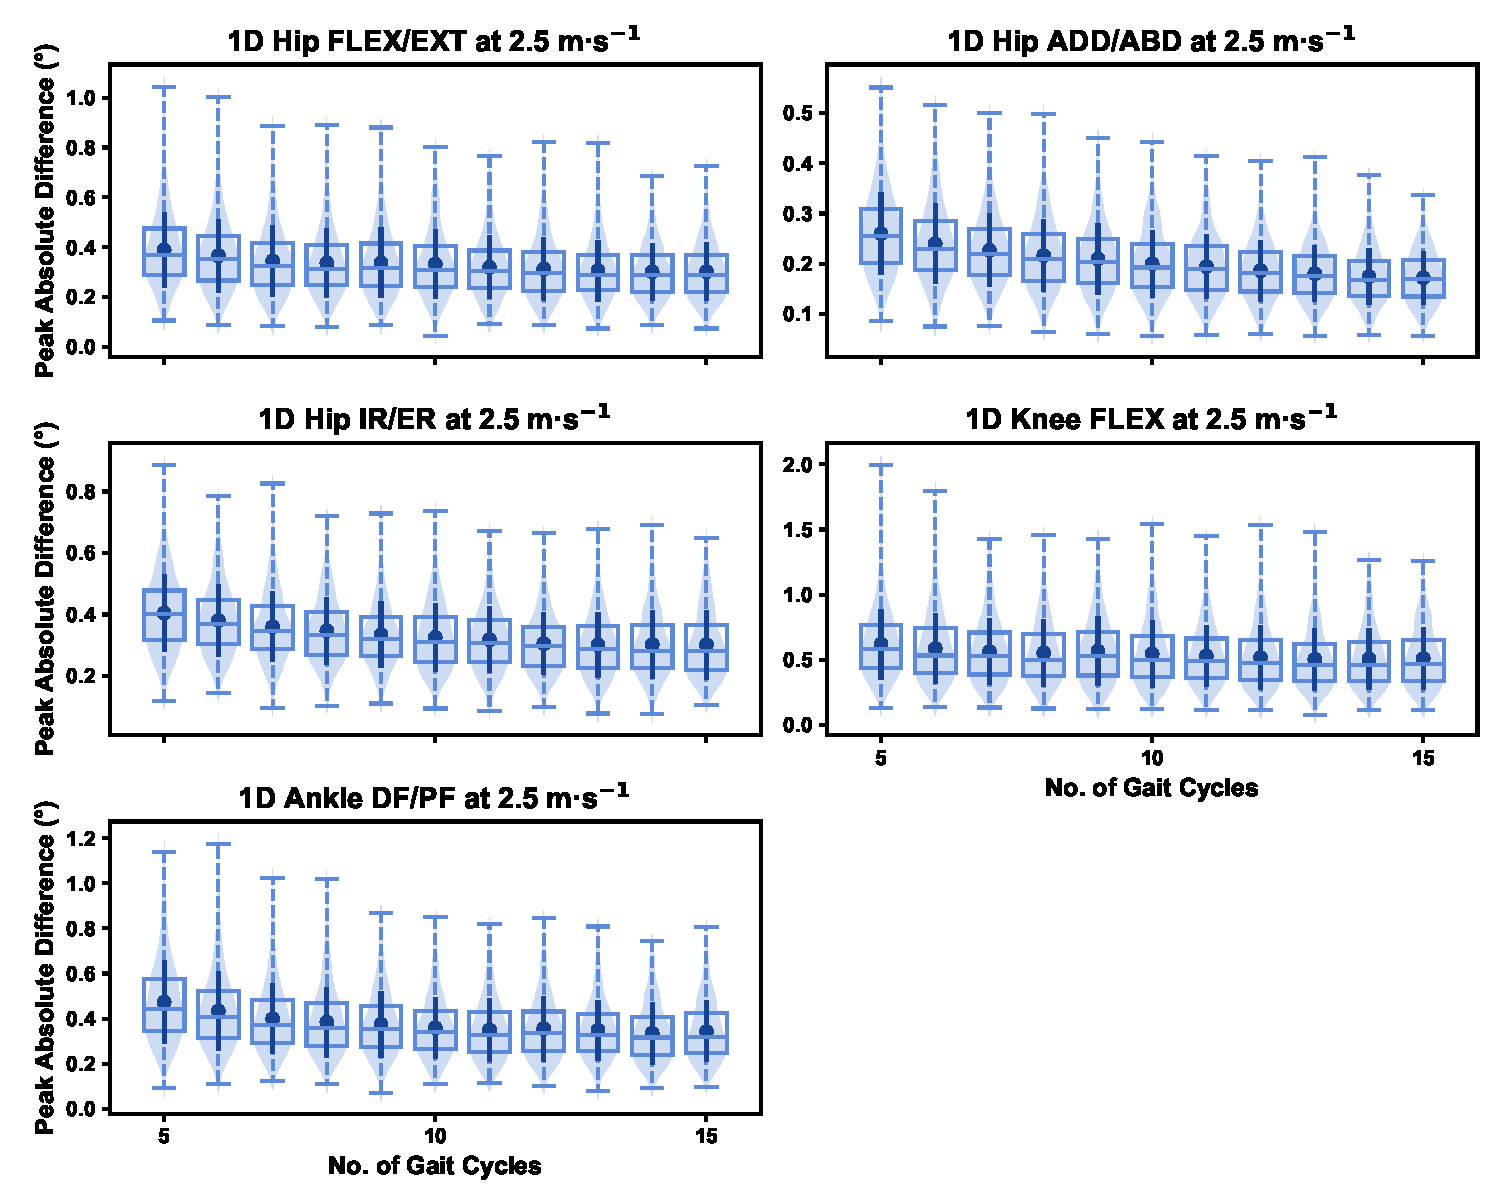
\includegraphics[width=1\linewidth]{D:/+GitRepos+/biomech-trial-selection/Analysis/GroundTruthComp/Figures/AbsoluteError_NoGaitCycle_runT25_1D} 

}

\caption{Peak absolute error in kinematic variables across the gait cycle (i.e. one-dimensional [1D]) when running at 2.5m·s$^{-1}$ using a subset of gait cycles versus all gait cycles from the 30 second treadmill bout. Horizontal lines within boxes equate to the median value, boxes indicate the 25$^{th}$ to 75$^{th}$ percentile, and whiskers indicate the range. Shaded violins are included to illustrate the distribution of values. FLEX — flexion; EXT — extension; ADD — adduction; ABD — abduction; IR — internal rotation; ER — external rotation; DF — dorsiflexion; PF — plantarflexion.}\label{fig:groundTruthError_runT25_1D}
\end{figure}

\begin{figure}

{\centering 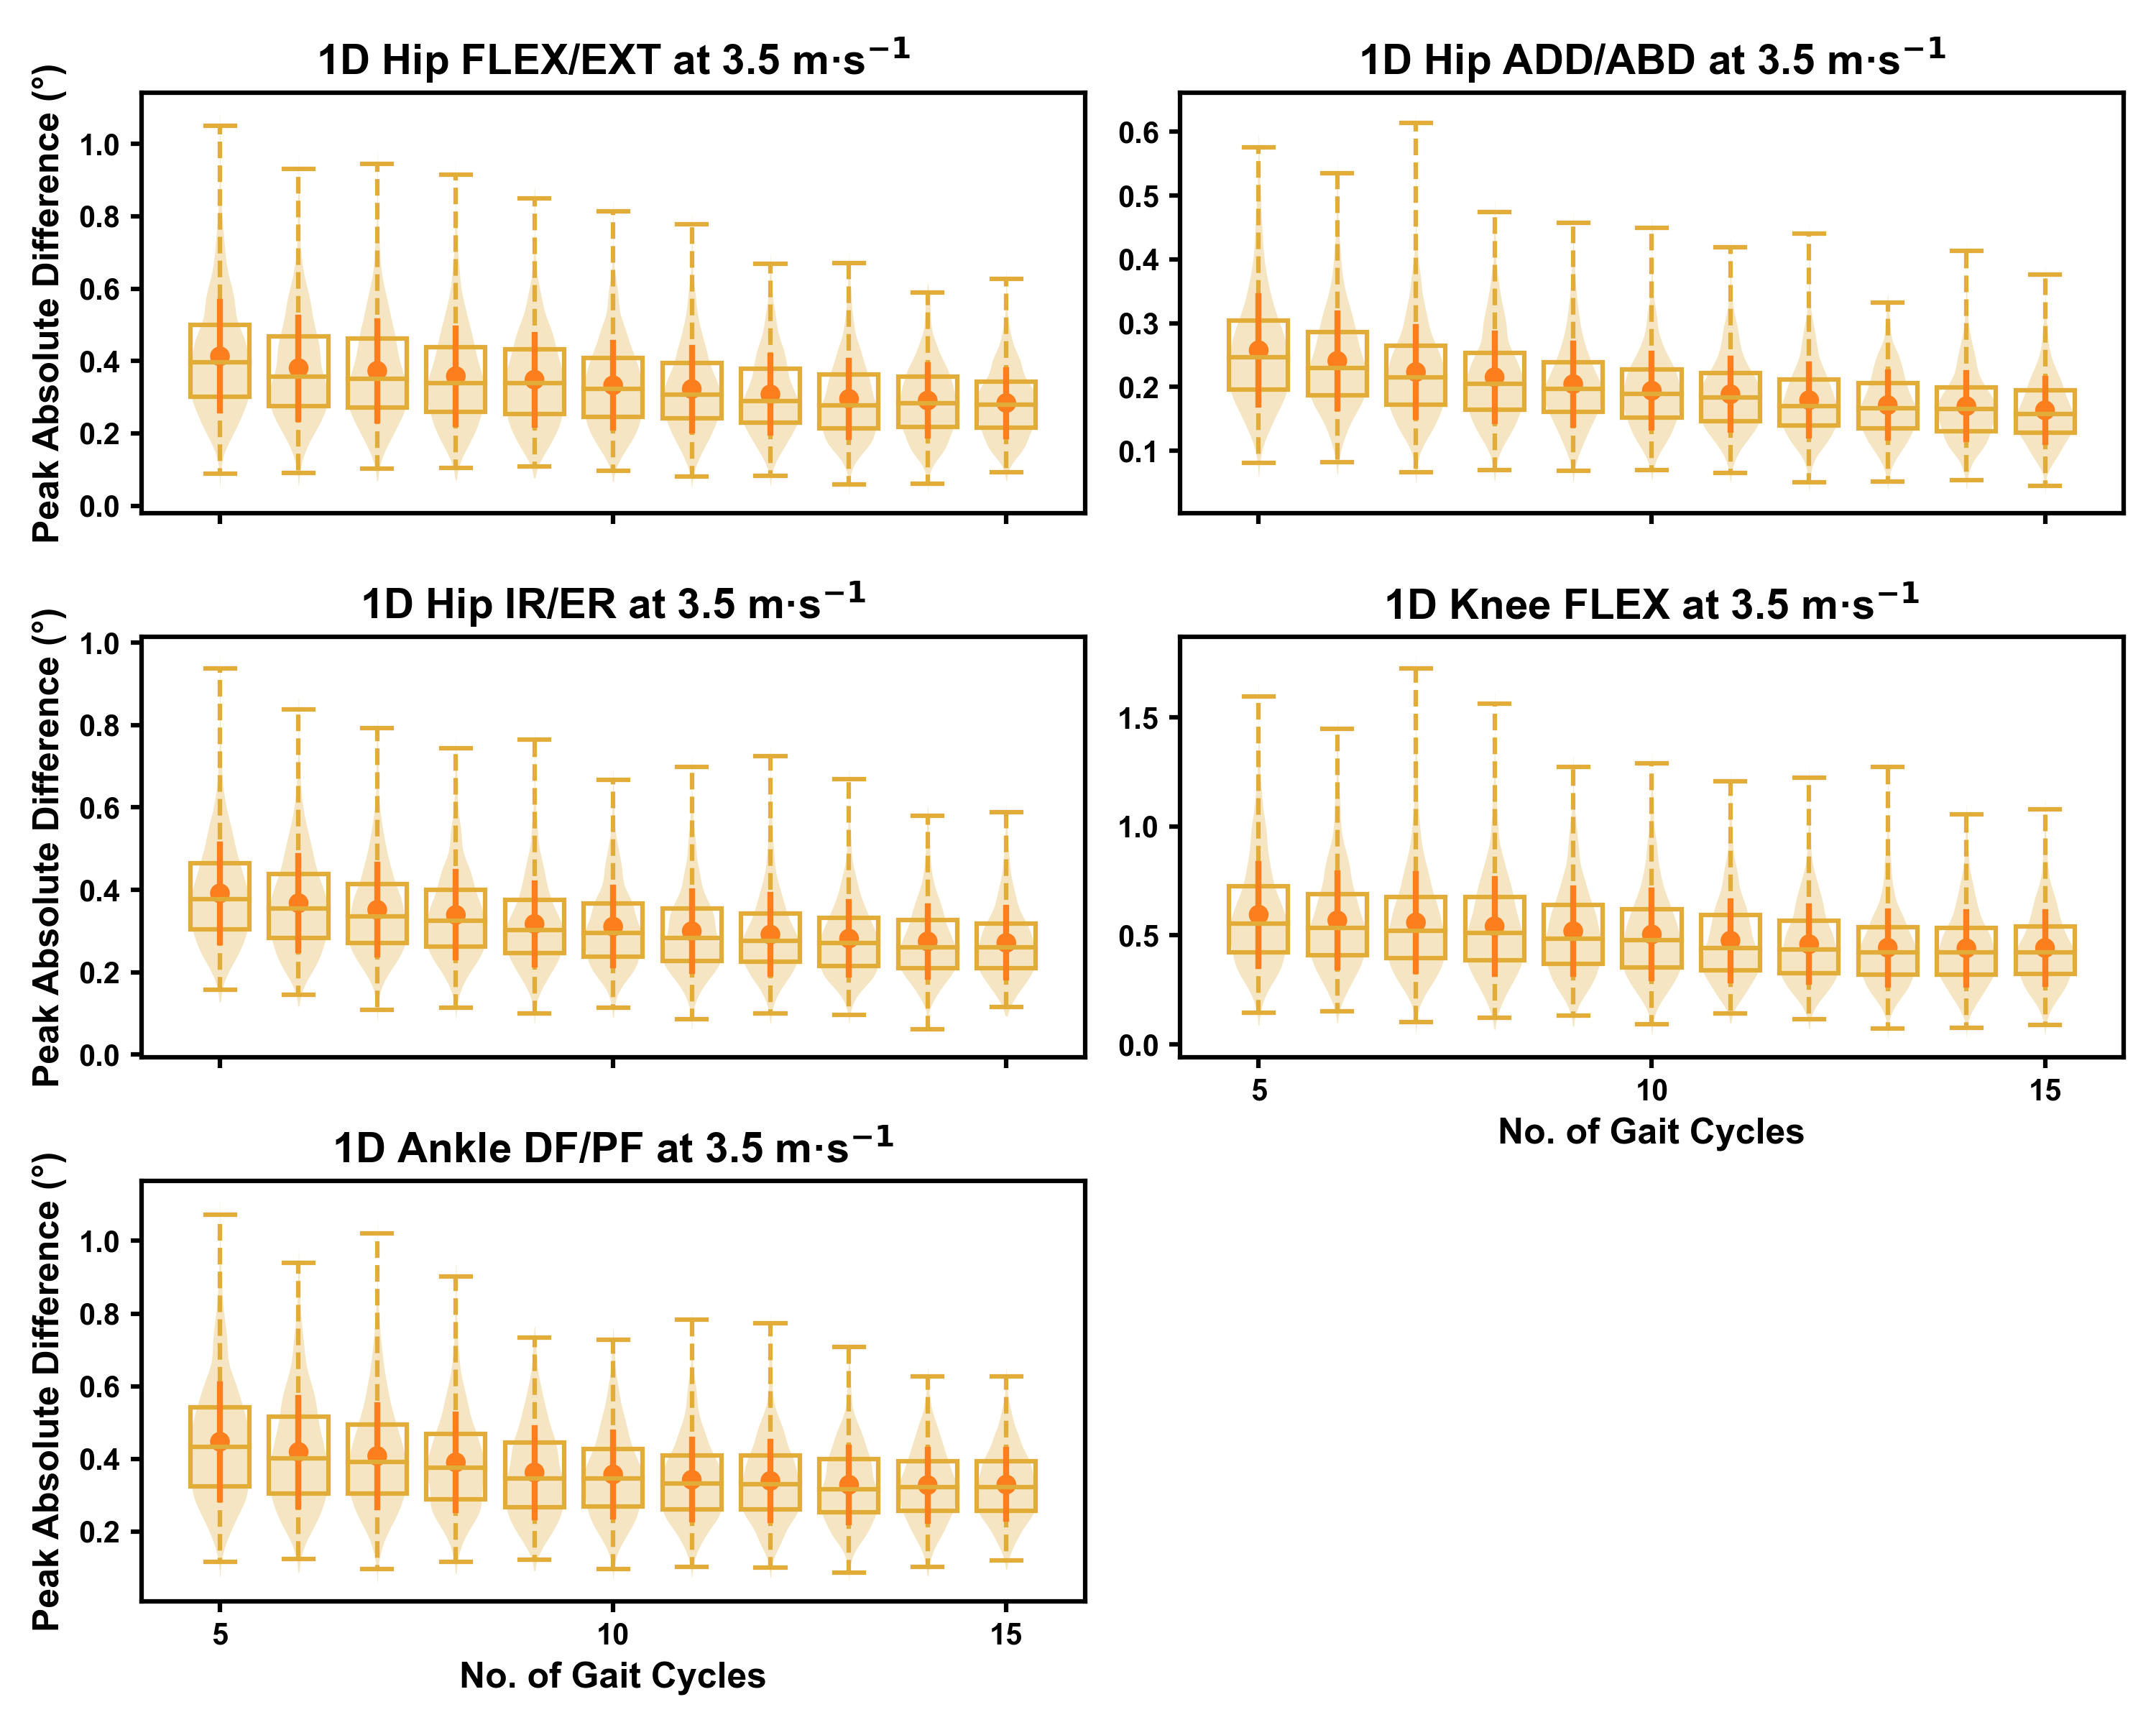
\includegraphics[width=1\linewidth]{D:/+GitRepos+/biomech-trial-selection/Analysis/GroundTruthComp/Figures/AbsoluteError_NoGaitCycle_runT35_1D} 

}

\caption{Peak absolute error in kinematic variables across the gait cycle (i.e. one-dimensional [1D]) when running at 3.5m·s$^{-1}$ using a subset of gait cycles versus all gait cycles from the 30 second treadmill bout. Horizontal lines within boxes equate to the median value, boxes indicate the 25$^{th}$ to 75$^{th}$ percentile, and whiskers indicate the range. Shaded violins are included to illustrate the distribution of values. FLEX — flexion; EXT — extension; ADD — adduction; ABD — abduction; IR — internal rotation; ER — external rotation; DF — dorsiflexion; PF — plantarflexion.}\label{fig:groundTruthError_runT35_1D}
\end{figure}

\begin{figure}

{\centering 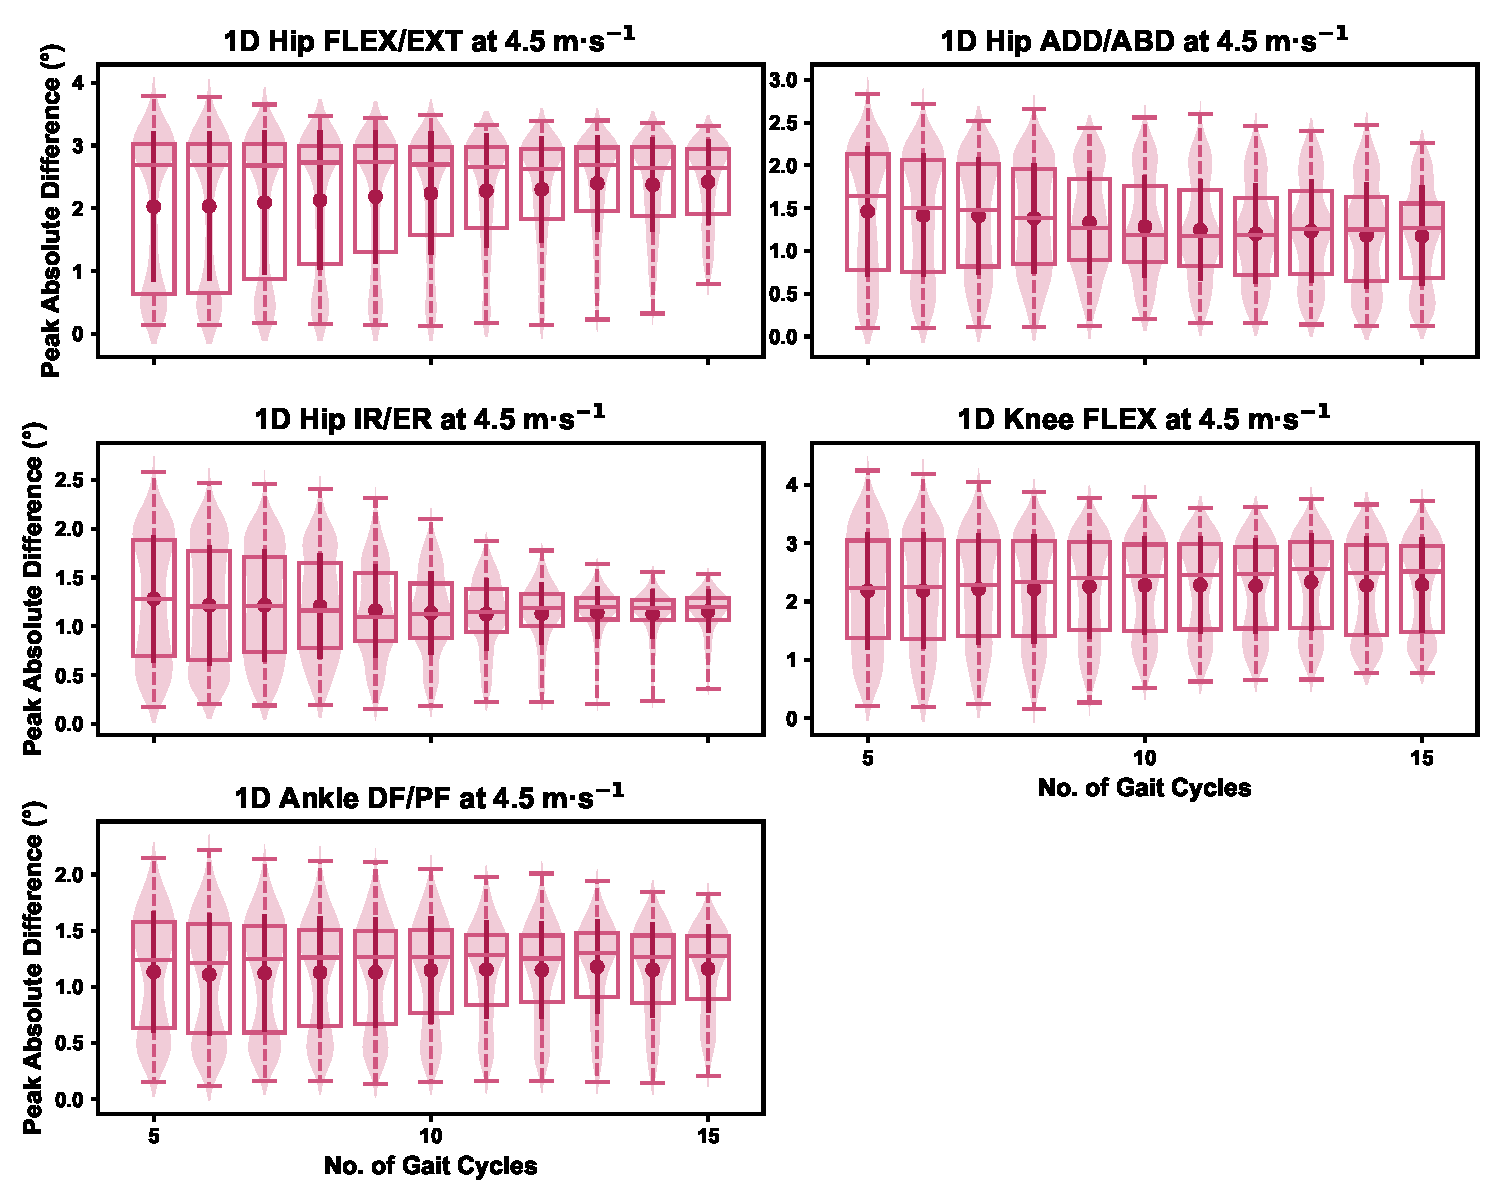
\includegraphics[width=1\linewidth]{D:/+GitRepos+/biomech-trial-selection/Analysis/GroundTruthComp/Figures/AbsoluteError_NoGaitCycle_runT45_1D} 

}

\caption{Peak absolute error in kinematic variables across the gait cycle (i.e. one-dimensional [1D]) when running at 4.5m·s$^{-1}$ using a subset of gait cycles versus all gait cycles from the 30 second treadmill bout. Horizontal lines within boxes equate to the median value, boxes indicate the 25$^{th}$ to 75$^{th}$ percentile, and whiskers indicate the range. Shaded violins are included to illustrate the distribution of values. FLEX — flexion; EXT — extension; ADD — adduction; ABD — abduction; IR — internal rotation; ER — external rotation; DF — dorsiflexion; PF — plantarflexion.}\label{fig:groundTruthError_runT45_1D}
\end{figure}

\ldots{}

\emph{TODO: Results here\ldots{}}

\begin{itemize}
\item
  The absolute error of the representative kinematic mean (compared to
  the mean from all cycles) progressively reduced as the number of gait
  cycles increased; but the errors were still quite small -- e.g.~0D at
  2.5 metres per second were all less than 1 degree
\item
  Errors for 0D did however become slightly larger with lower gait cycle
  numbers at the highest running speed, and typically needed to use a
  high number (e.g.~30) gait cycles to reach similar levels of error
  compared to the `ground truth' during the 4.5 metres per second
\item
  The peak absolute errors from the 1D comparison showed a similar trend
  of reducing with a greater number of gait cycles, but errors were
  similarly small
\item
  Wasn't as an obvious jump with higher running speed in the peak
  absolute errors for 1D comparisons
\end{itemize}

\hypertarget{how-does-the-sampling-location-within-a-treadmill-bout-impact-the-representative-kinematic-mean}{%
\section{How does the sampling location within a treadmill bout impact
the representative kinematic
mean?}\label{how-does-the-sampling-location-within-a-treadmill-bout-impact-the-representative-kinematic-mean}}

\emph{TODO: add methods\ldots{}}

\ldots{}

\emph{TODO: add results\ldots{}}

\begin{itemize}
\tightlist
\item
  Increasing the number of gait cycles didn't really change the errors
  between the sampling means
\item
  Errors between sampling sections were relatively small for 2.5 and 3.5
  metres per second, but increased a little for 4.5 metres per second.
\item
  Effectively at lower speeds, where you sample your gait cycles from in
  a period of treadmill running didn't have a dramatic effect on the
  kinematic mean at 2.5 and 3.5 metres per second (i.e.~with 1 degree of
  one another), but this slightly increased at the highest running speed
\item
  Practically what this means is you can expect a little bit of error
  depending on where the data is sampled from, but not a whole lot; and
  this isn't really modulated from a number of gait cycles perspective
\end{itemize}

\hypertarget{results}{%
\section{Results}\label{results}}

\begin{verbatim}
##      speed           dist       
##  Min.   : 4.0   Min.   :  2.00  
##  1st Qu.:12.0   1st Qu.: 26.00  
##  Median :15.0   Median : 36.00  
##  Mean   :15.4   Mean   : 42.98  
##  3rd Qu.:19.0   3rd Qu.: 56.00  
##  Max.   :25.0   Max.   :120.00
\end{verbatim}

\hypertarget{discussion}{%
\section{Discussion}\label{discussion}}

\ldots{}

\textbf{\emph{KEY POINT = higher speeds seem to necessitate a greater
number of gait cycles to reach stability and be representative of the
entire running bout}}

\textbf{\emph{KEY POINT = despite seeing improvements in the `error' of
a representative kinematic mean with a larger number of gait cycles, the
differences were quite small (e.g.~1-2 degrees at a maximum). This may
be important to detect small differences in running technique, but the
magnitude of some of these errors perhaps need to be considered against
the added data collection, management, and processing times associated
with including more gait cycles. For example, your representative mean
for knee flexion may improve by 0.5 degrees when going from 5 to 30 gait
cycles --- but how much extra time does this take, data storage too?
Effectively a small number of cycles sampled from a longer continuous
treadmill bout presents a relatively similar kinematic mean compared to
a mean calculated from the entire bout of running.}}

\textbf{\emph{KEY POINT = once you've decided how many gait cycles
you're using, where do you take the data from? Our results suggest it
probably doesn't matter too much, and this opinion doesn't really change
if you're using more or less gait cycles to create the mean. If you are
taking a sub-sample from the treadmill bout, you can expect this to have
a potential effect within the realm of \textless{} 1 degree at lower
speeds -- but slightly higher at faster speeds. Practically what this
means is if you see a very small difference between conditions, groups
etc., this could simply be driven by the sampling from the treadmill
bout (e.g.~if you sampled from a different portion, could the results be
different?). Note that we sampled consecutiv gait cycles for this
analysis.}}

Stability analysis -- reveals for entire 1D spectrum to be `stable' in
accordance with existing definitions (i.e.~within 0.25 SD), 30 gait
cycles may be necessary for capture; whereas we saw a similar values for
0D variables to Oliveira study with around 20 required for these
variables. Unsurprisingly, relaxing the bounds as to what is considered
`stable' (i.e.~from 0.25SD up to 1SD) resulted in less gait cycles being
required for a stable pattern

There was no noticeable effect across different kinematic variables for
the number of cycles to reach stability; there was a potential small
increase in the number of cycles required for achieving `stability' as
running speed increased. It took more gait cycles for stability to be
reached across the majority of participants with higher running speeds
-- consideration for research at higher speeds

Our fourth question perhaps presents the most practically meaningful
analysis of this work, in understanding how the number and selection of
gait cycles could impact the conclusions of a comparative study using a
paired design\ldots{}


\end{document}

